\section{Exercise and Report}
\subsection{Voltage Follower}
Voltage follower is one of the simplest uses of an operational amplifier, where the output
voltage is exactly same as the input voltage applied to the circuit. In other words, the gain
of a voltage follower circuit is unity. The connections are proposed as follows:
\begin{figure}[h]
    \centering
    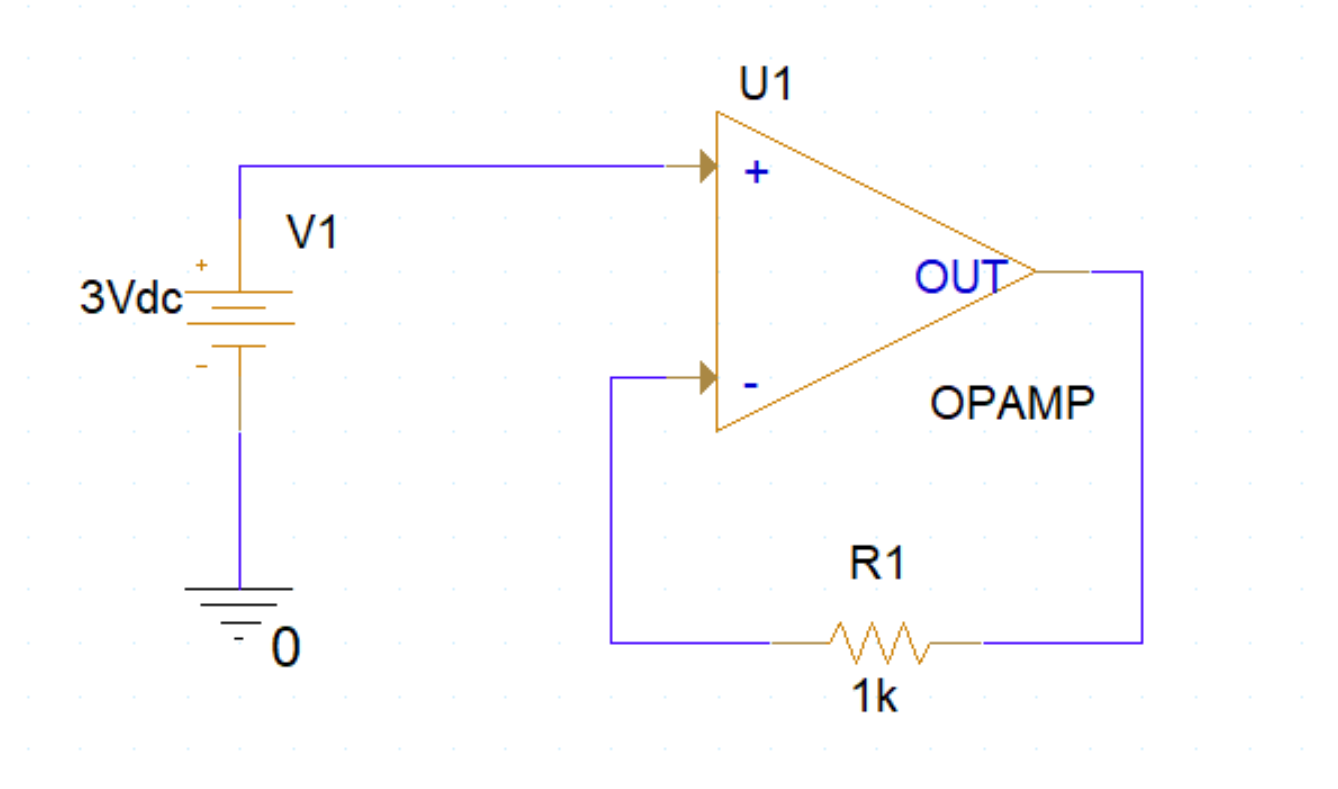
\includegraphics[width=0.6\textwidth]{graphics/ex1/f1.png}
    \caption{ Opamp follower circuit}
\end{figure}

A voltage follower has low output impedance and extremely high input impedance, and
this makes it a simple and effective solution to problematic impedance relationships.

If
a high-output-impedance sub-circuit must transfer a signal to a low-input-impedance
sub-circuit, a voltage follower placed between these two sub-circuits will ensure that the
full voltage is delivered to the load.

\textbf{Ảnh mô phỏng}

\begin{figure}[ht]
    \centering
    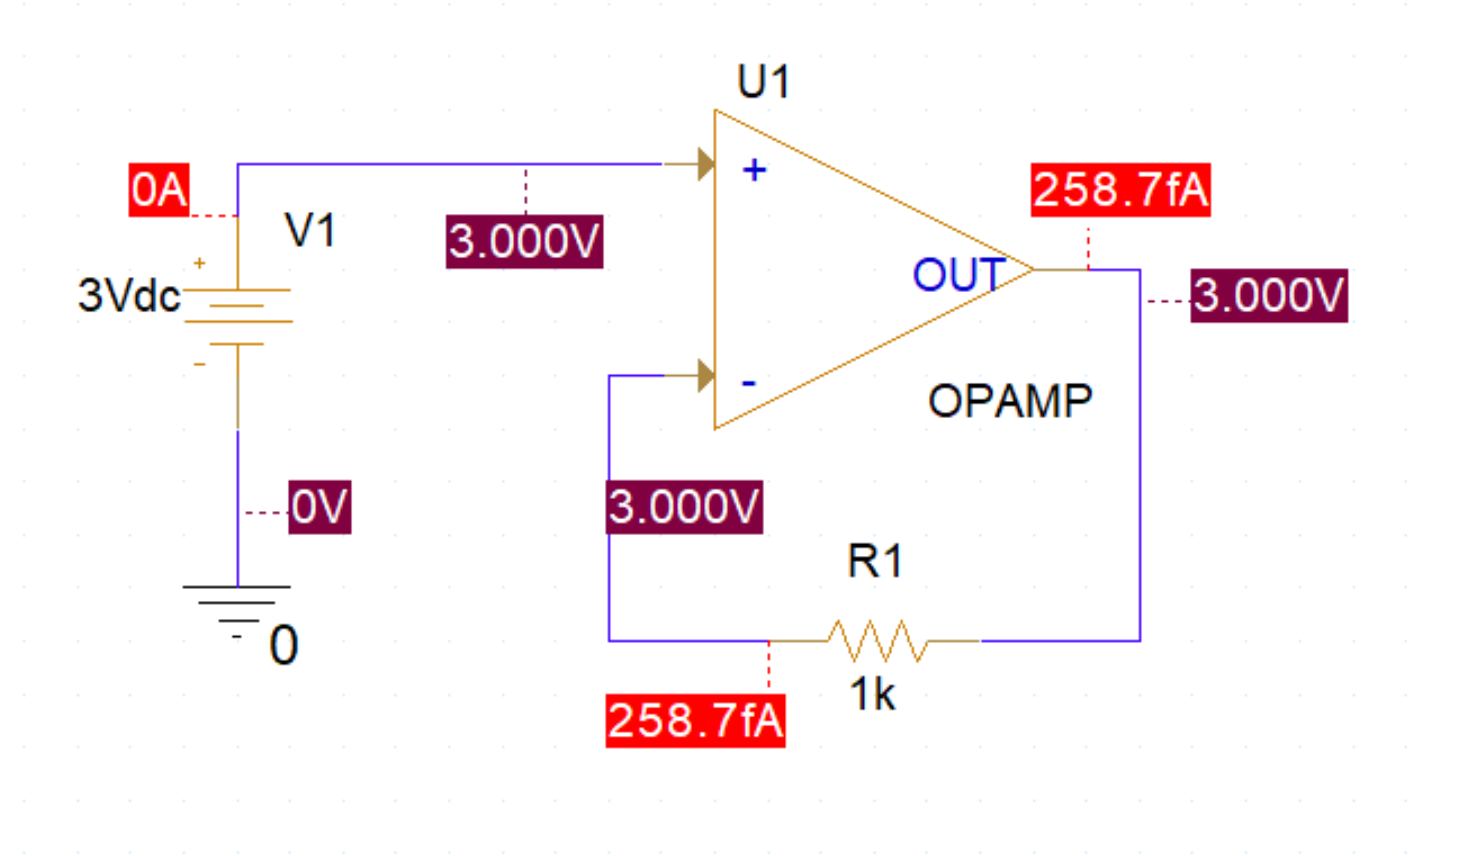
\includegraphics[width=0.6\textwidth]{graphics/ex1/f2.png}
    \caption{Simulation Opamp follower circuit with $R_1 = 1k \Omega$ }
\end{figure}

\begin{figure}[ht]
    \centering
    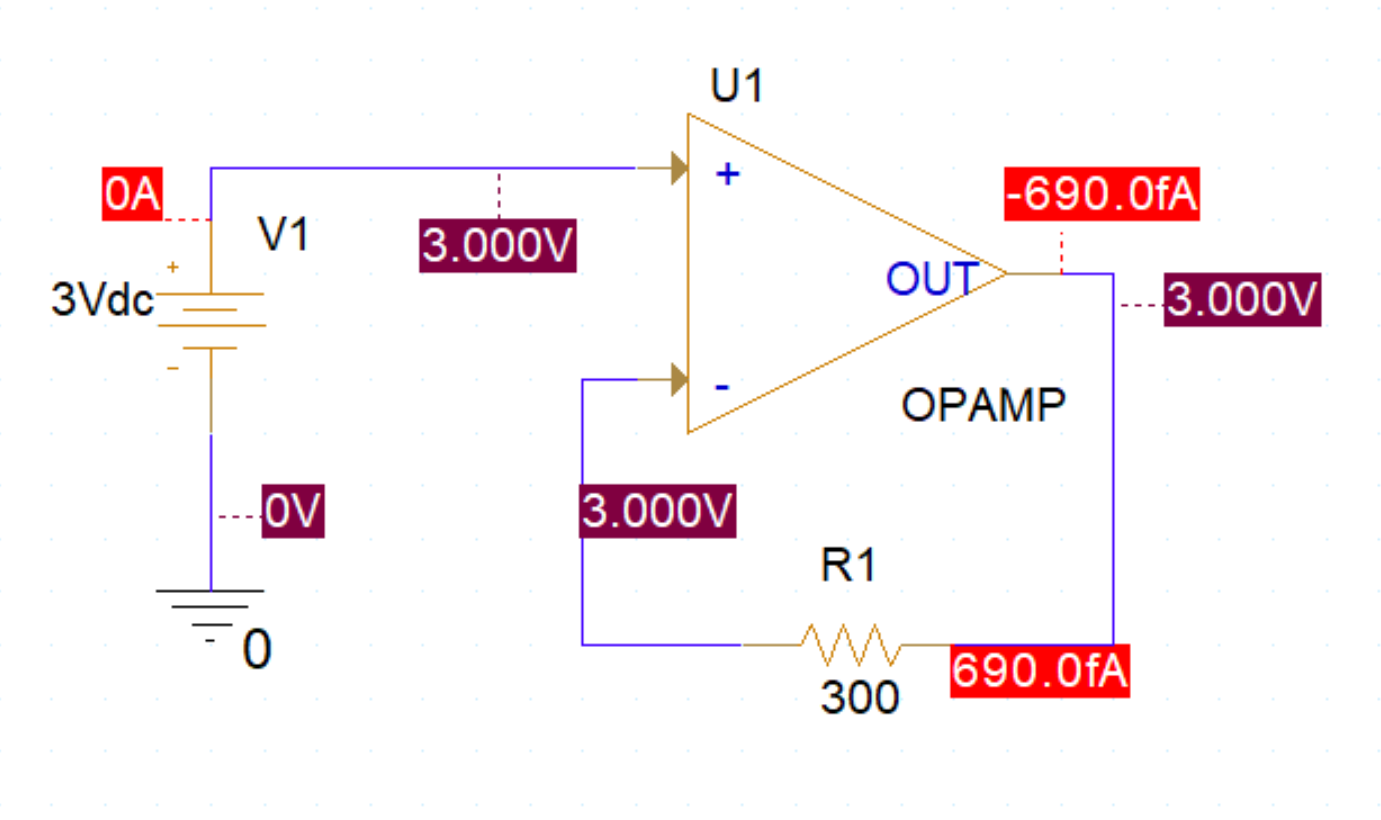
\includegraphics[width=0.6\textwidth]{graphics/ex1/f3.png}
    \caption{Simulation Opamp follower circuit with $R_1 = 300 \Omega$}
\end{figure}

Ta có mạch tương đương của Opamp như sau:

\begin{figure}[ht]
    \centering
    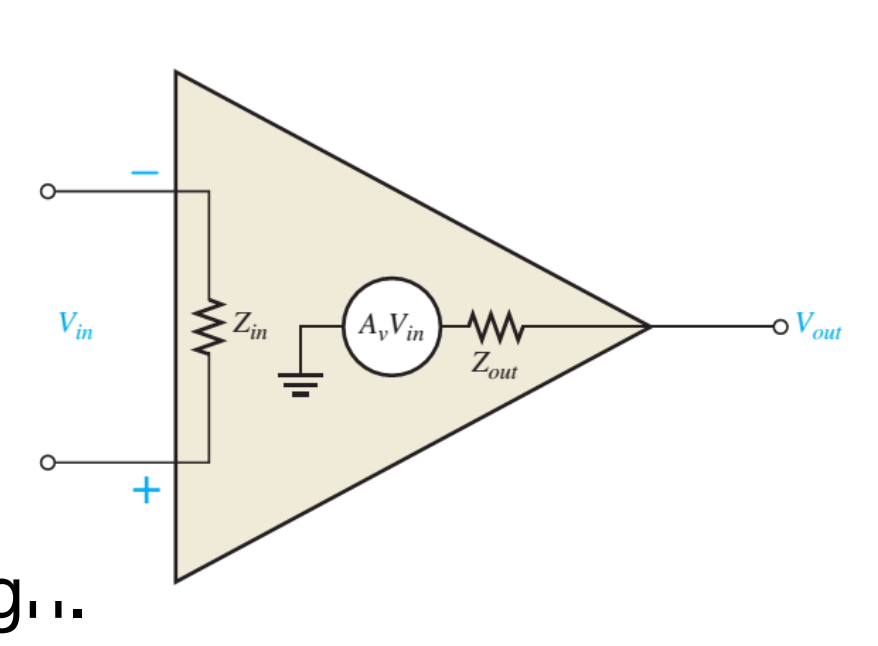
\includegraphics[width=0.6\textwidth]{graphics/ex1/f4.png}
    \caption{Mô hình thực tế của Opamp}
\end{figure}

Theo định luật Ohm, ta có: $I = \dfrac{V_{out} - V^+}{R_1 + Z_{in}}$

Mà trở kháng đầu vào ($Z_{in}$) rất lớn nên $I \approx 0$. Do vậy $V_{out} \approx V^+$ với bất cứ giá trị nào của $R_1$.
\pagebreak
\subsection{High-Current Voltage Follower}
The voltage follower's low output impedance makes it a good circuit for driving current
into a low-impedance load, but it's important to remember that most op-amps are not
designed to deliver large output currents. The most basic circuit for buffering an op-amp's
output current is the following:

\begin{figure}[ht]
    \centering
    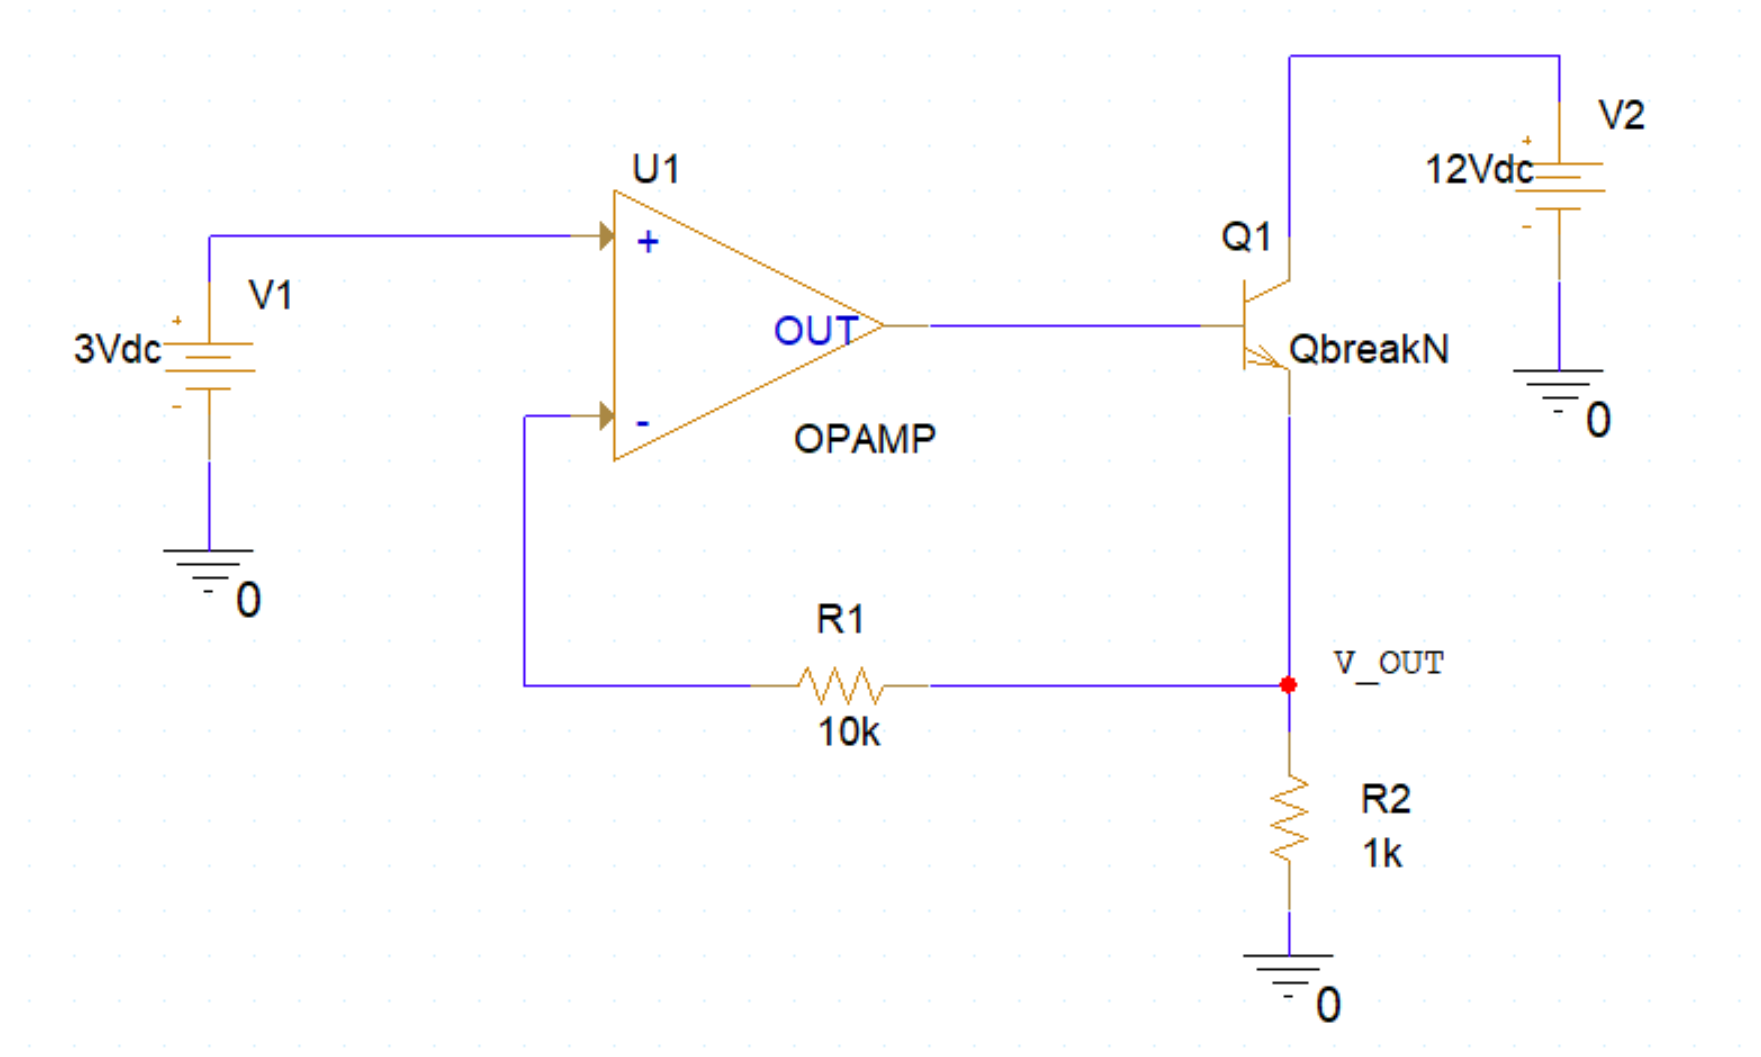
\includegraphics[width=0.8\textwidth]{graphics/ex1/f6.png}
    \caption{Opamp follower circuit}
\end{figure}

The voltage at the positive pin of the Opamp is copied to VOUT . In this schematic, R2 is
used to simulate a load device, which can be a motor or an high power LED. However, in
this case, there is a high current can pass the load.

\textbf{Ảnh mô phỏng}

\begin{figure}[ht]
    \centering
    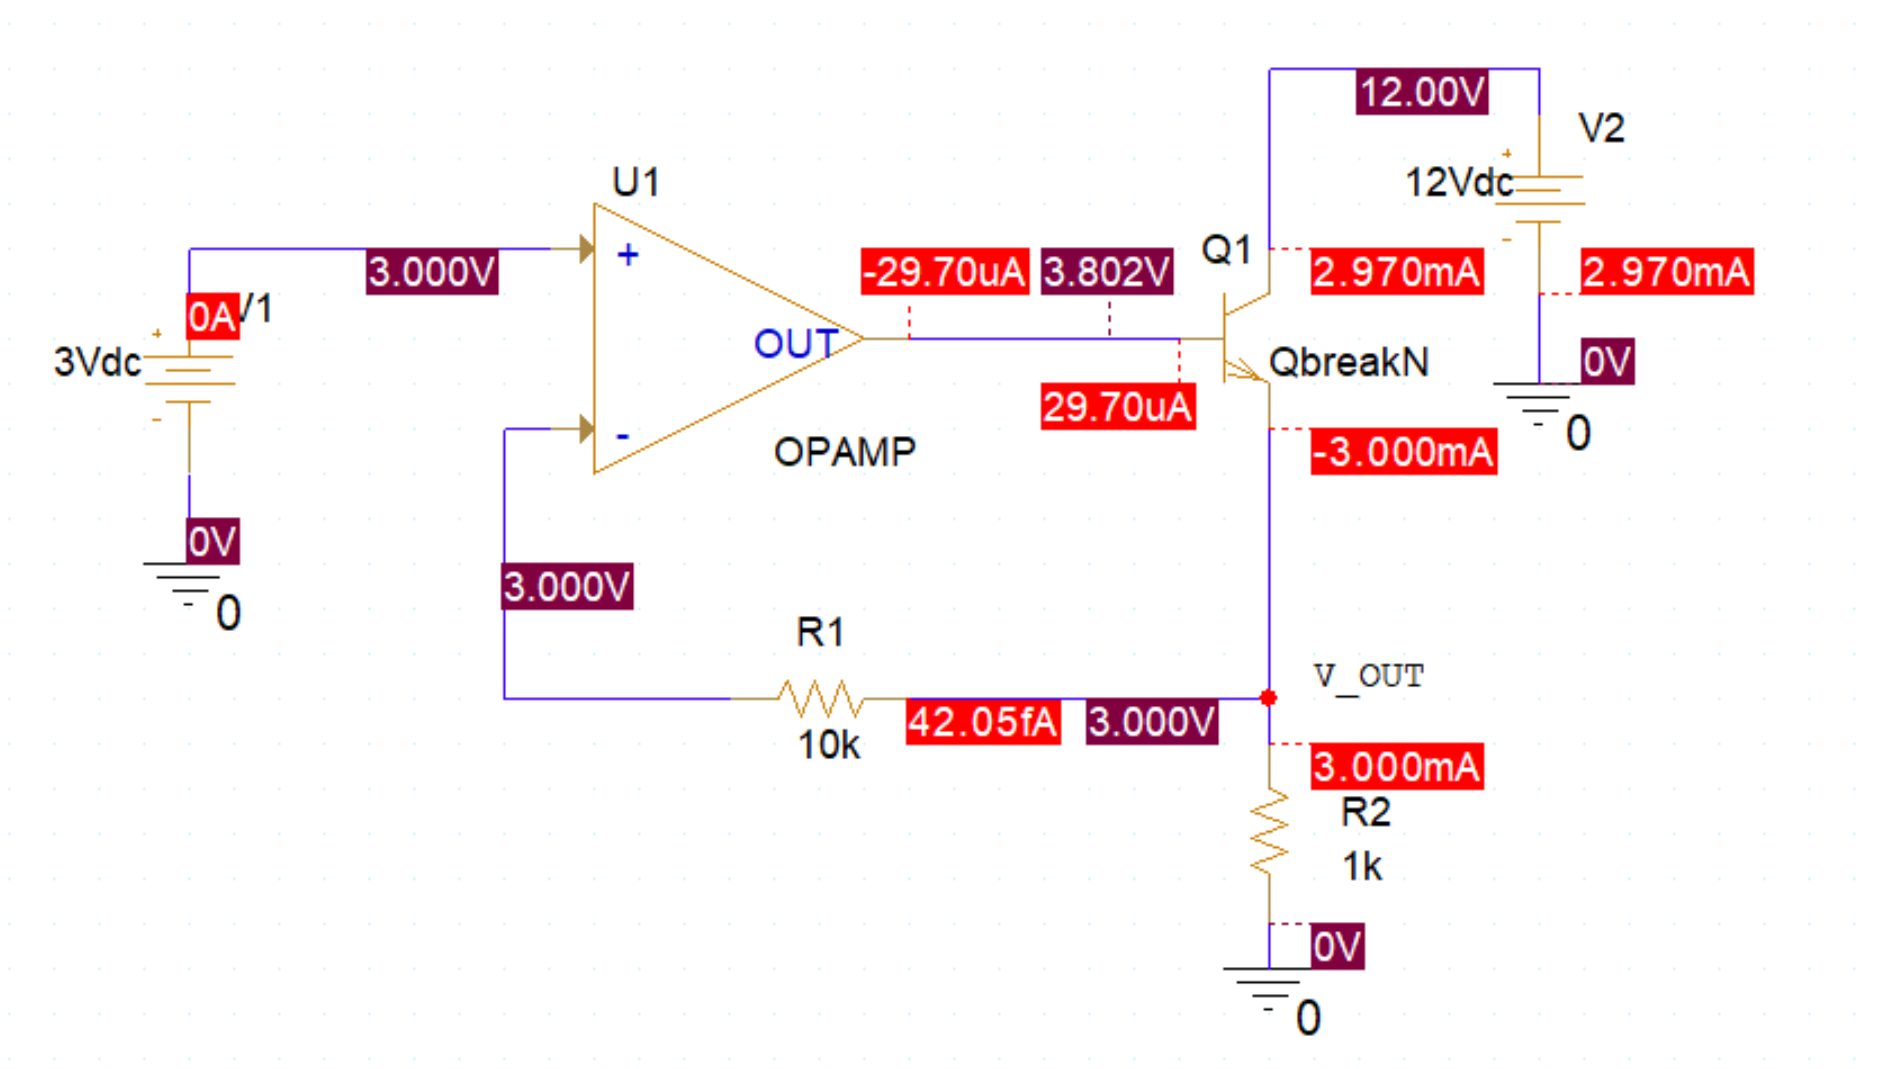
\includegraphics[width=1\textwidth]{graphics/ex1/f5.png}
    \caption{Simulation Opamp follower circuit}
\end{figure}
\pagebreak

Theo định luật Ohm, ta có: $I_{R_1} = \dfrac{V_{out} - V^+}{R_1 + Z_{in}}$

Mà trở kháng đầu vào ($Z_{in}$) rất lớn nên $I_{R_1} \approx 0$. Do vậy $V_{out} \approx V^+$ với bất cứ giá trị nào của $R_1$.

Với $V_{out} = V^+ = 3 V$, theo định luật Ohm: $I_{R_2} = \dfrac{V_{out}-0}{R_2} = 3 $ (mA).

Giả sử BJT ở vùng tích cực, $V_{BE} \approx 0.7$ V (Trong mô phỏng trên PSpice $V_{BE} \approx 0.8$ V) và $I_B = \beta I_C$ (Trong mô phỏng PSpice $\beta = 100$)

Do vậy, điện áp tại đầu ra của Opamp: $V_{Opamp\_out} = V_{BE} + V_{out} = 0.8 + 3 = 3.8 $ V và

$I_{R_2} = I_B + I_C = (1 + \beta)I_B = 101I_B \rightarrow I_B = \frac{I_{R_2}}{101} = 29.7(\mu A)$ và $I_C = 100I_B = 2.97$ (mA).
\pagebreak
\subsection{Voltage Follower with Gain}
This basic circuit is not limited to the unity-gain configuration. As with a non-buffered
op-amp, you can insert resistors into the feedback path to create overall gain from the
input to the load voltage. Here is the non-unity-gain version of the circuit:
Students are proposed to implement this circuit on PSPICE with input is 2V and the gain
is 3. The voltage supply for the load side is 12VDC. Value of RLOAD is 1K.

\begin{figure}[ht]
    \centering
    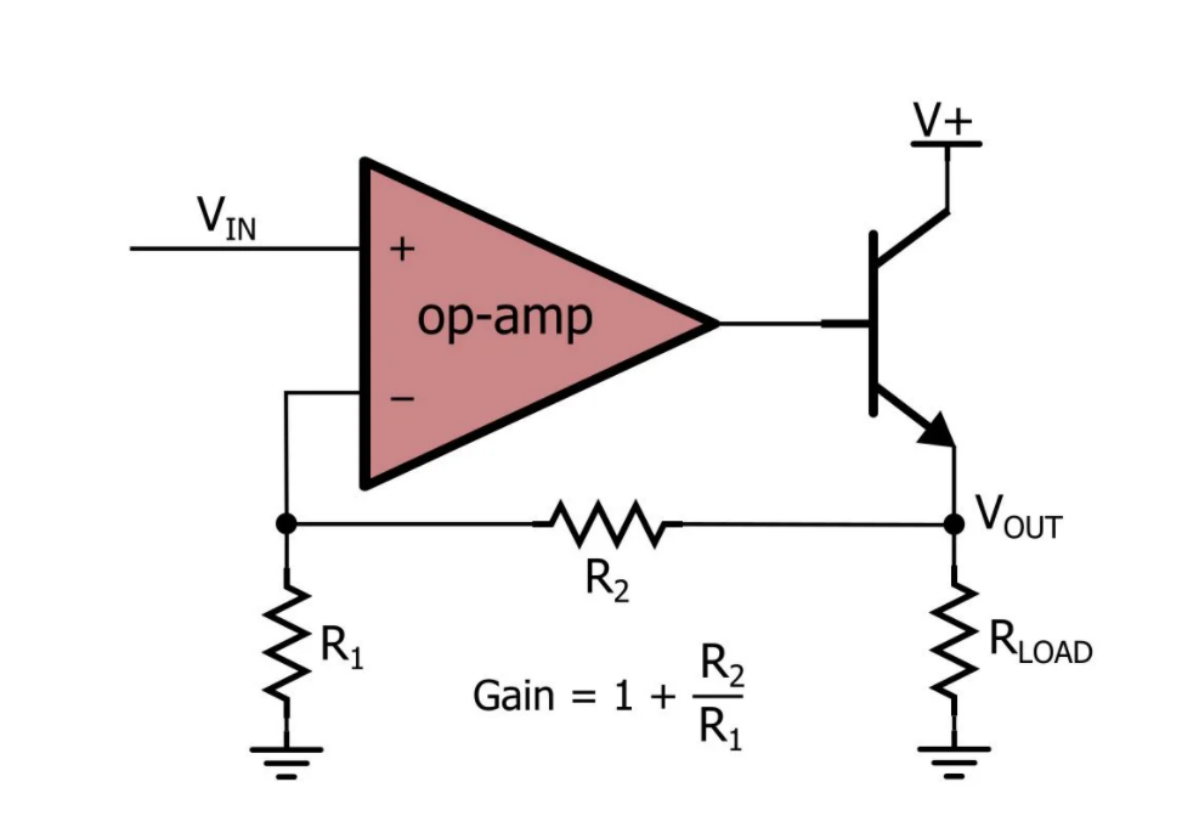
\includegraphics[width=0.5\textwidth]{graphics/ex1/f7.png}
    \caption{Opamp follower with gain for the output}
\end{figure}

\textbf{Ảnh mô phỏng}

\begin{figure}[ht]
    \centering
    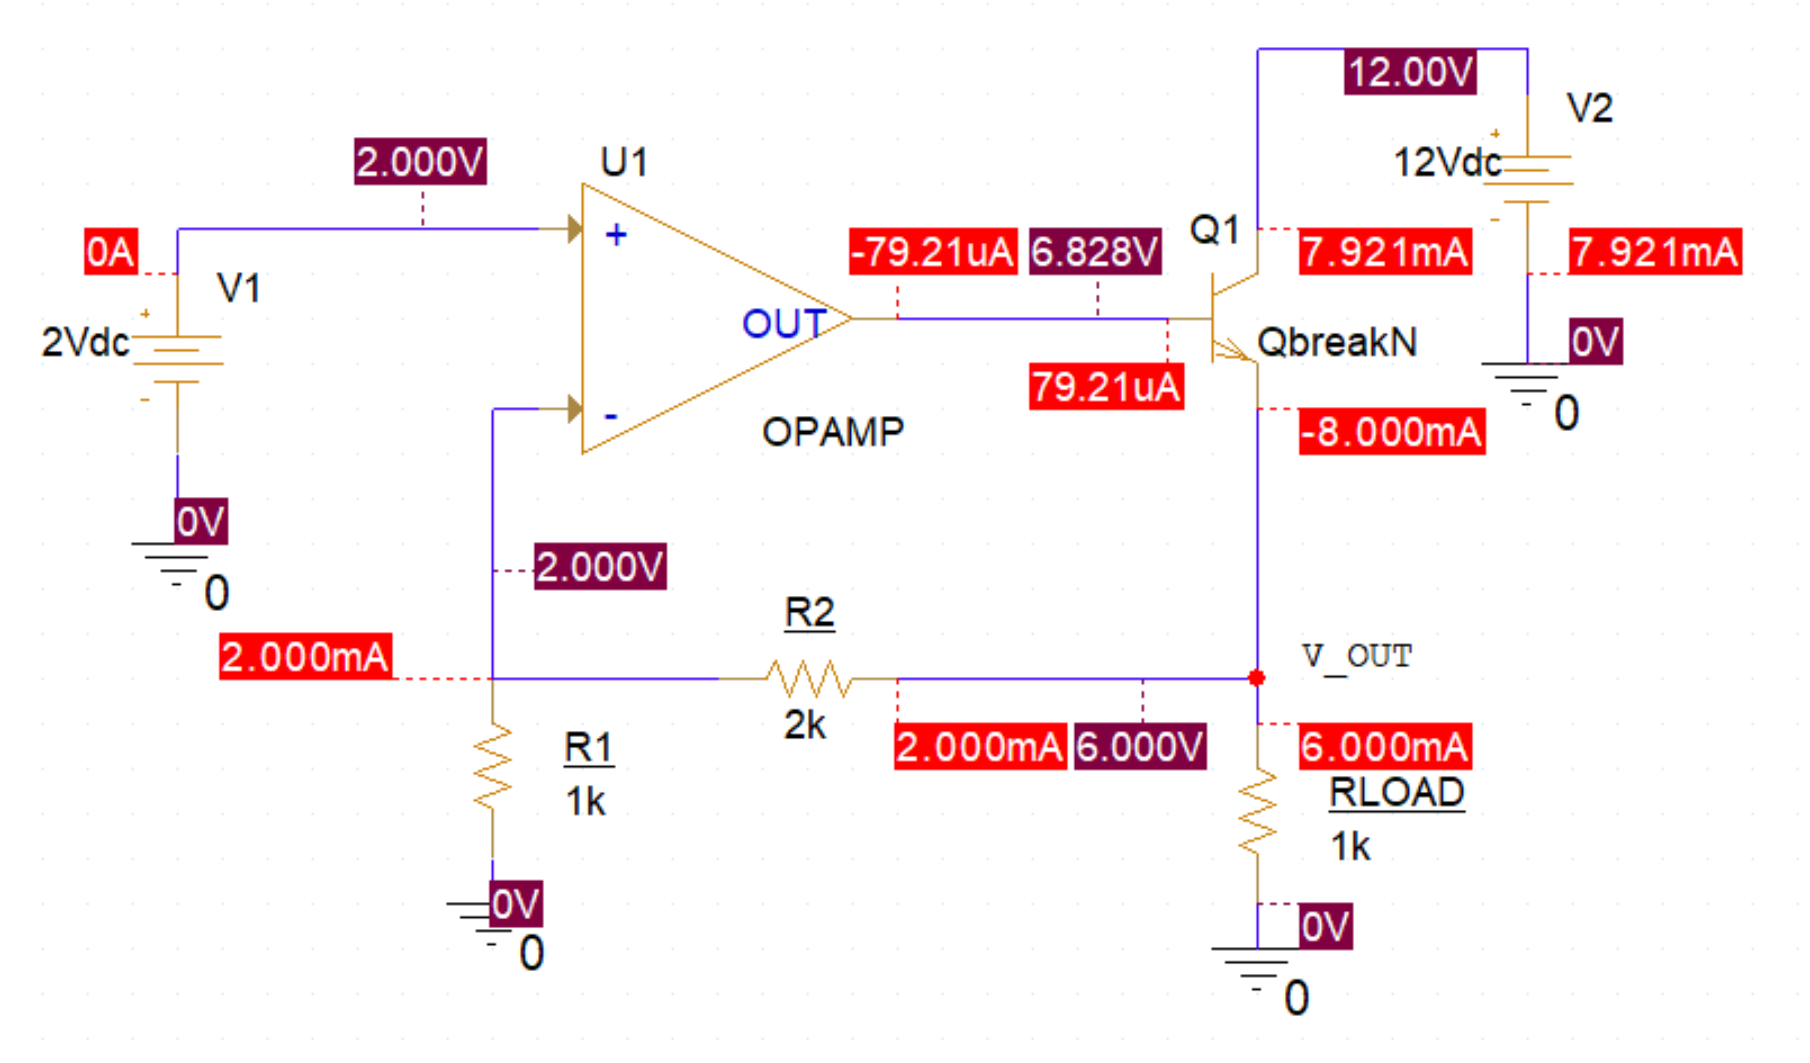
\includegraphics[width=0.95\textwidth]{graphics/ex1/f8.png}
    \caption{Opamp follower with gain for the output}
\end{figure}

Ta có, Opamp hồi tiếp âm do điện trở đầu vào lớn nên $V^+ = V^- = 2$ V

Mà $I_{Opamp^-} \approx 0$ nên $I_{R_1} = I_{R_2} = \dfrac{V^- - 0}{R_1} = \dfrac{V^+}{R_1}$

Theo định luật Ohm,  $I_{R_2} = \dfrac{V_{out} - V^-}{R_2} \rightarrow V_{out} = V^- + I_{R_2}R_2 = V^+ + \dfrac{V^+R_2}{R_1} = V^+(1 + \dfrac{R_2}{R_1})$

Hay $V_{out} = (1 + \dfrac{R_2}{R_1})V_{in} \rightarrow GAIN = \dfrac{V_{out}}{V_{in}} = 1 + \dfrac{R_2}{R_1}$.

Trong mô phỏng lấy ví dụ $R_1 = 1k$ và $R_2 = 2k$ để được GAIN = 3. Như vậy, ta có $V_{out} = 2.3 = 6$ (V).

Theo định luật Ohm, $I_{R_{LOAD}} = \dfrac{V_{out}}{R_{LOAD}} = \dfrac{6}{1k} = 6 $ (mA).

$V_{OPAMP\_out} = V_{BE} + V_{out} = 6 + 0,8 = 6,8$ (Trong mô phỏng lấy $V_{BE} \approx 0.8$ V) và

$I_{out} = I_{R_2} + I_{R_{LOAD}} = \frac{V_{in}}{R_1} + 6$ = 8 (mA)

$I_{out} = (1+\beta)I_B  = 101I_B \rightarrow I_B = 79,2 (\mu A) \rightarrow I_C = 100I_B = 7,92$ (mA) (Trong mô phỏng $\beta$ của BJT = 100)
\pagebreak
\subsection{Summing Amplifier}
Students are proposed to implement following schematic in PSPICE and run the simulation with R1 = 1K, R2 = 2K, R3 = 5K, Rf = 9K, Ri = 1K. There inputs are V1 = 1V, V2 = 2V and
V3 = 3V. This circuit is a non inverting summing configuration using opamp.

\begin{figure}[ht]
    \centering
    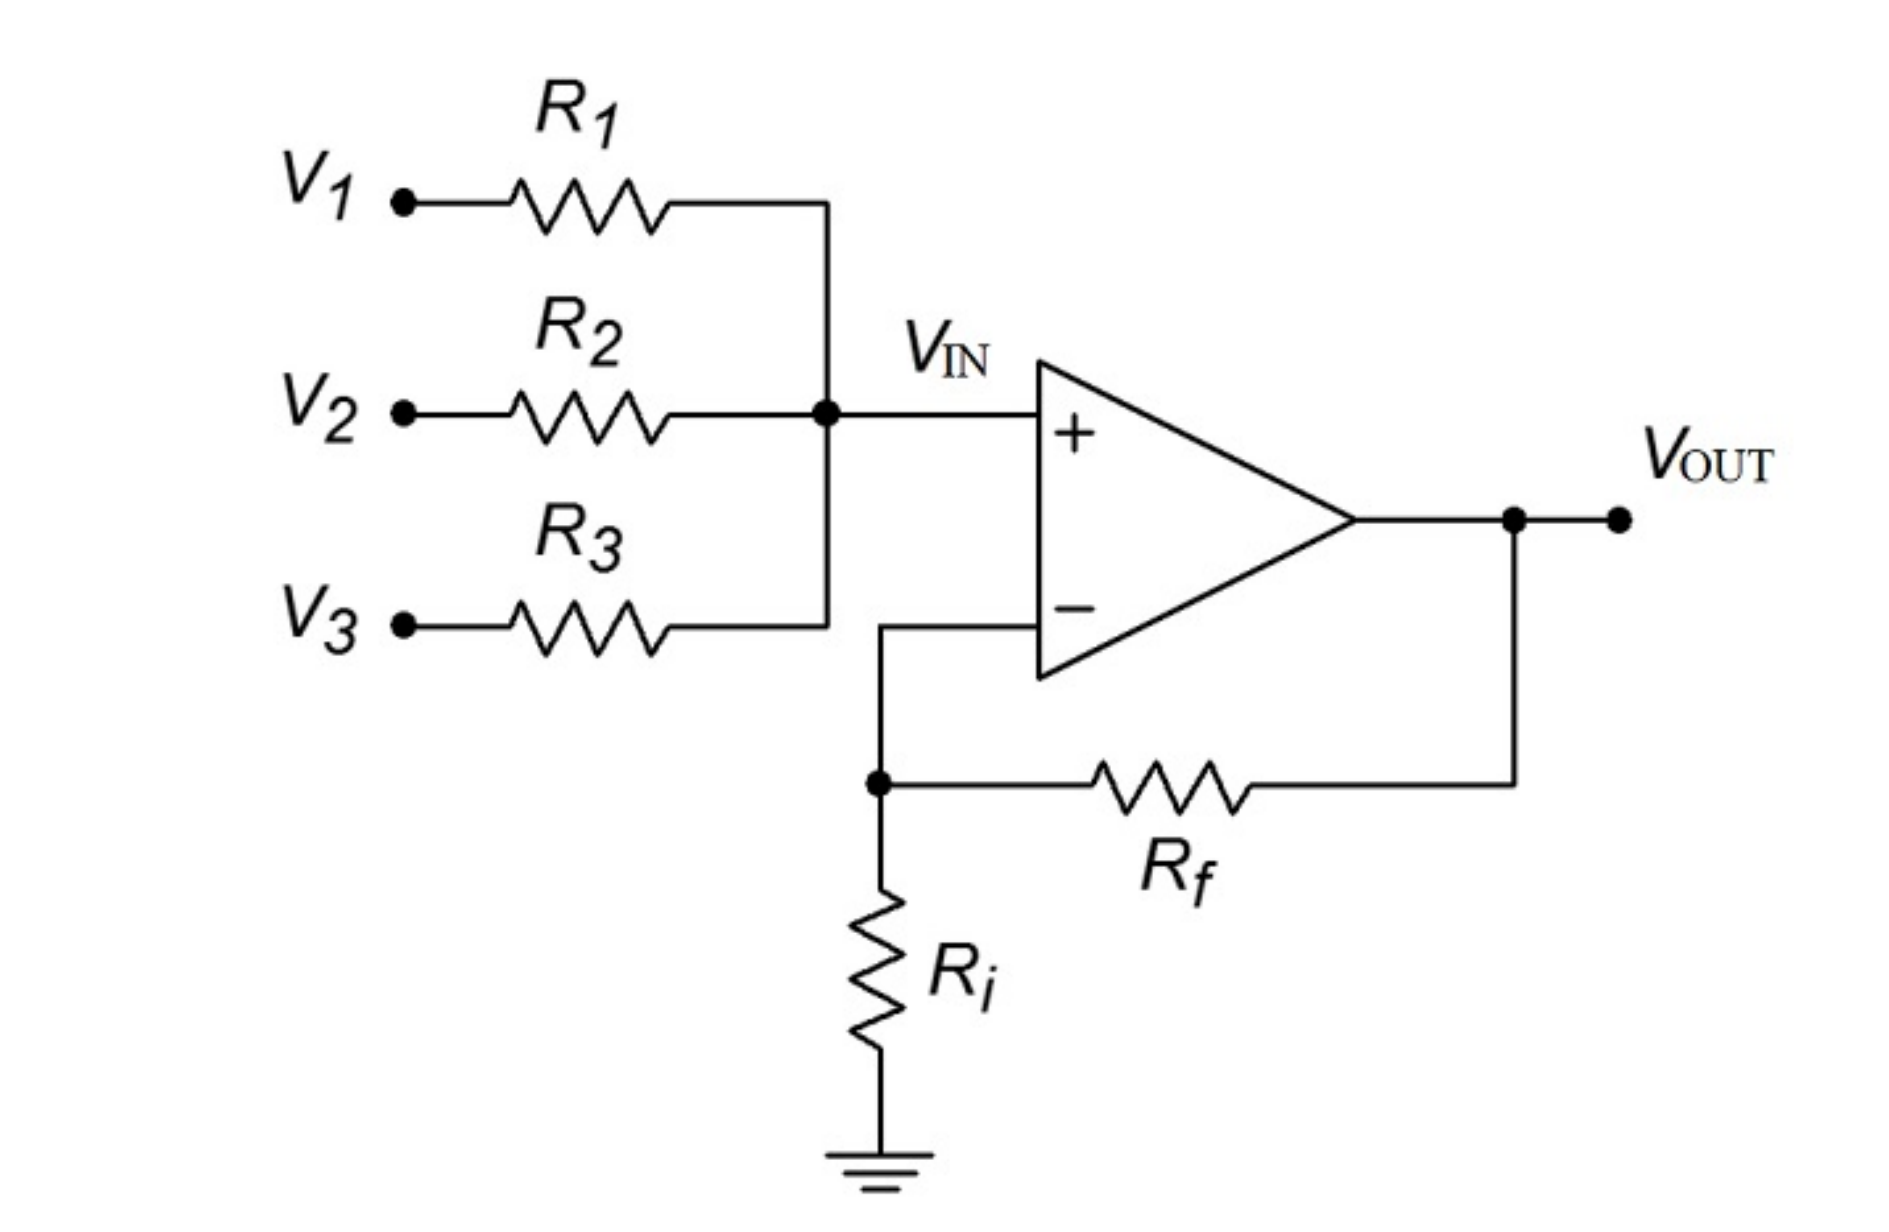
\includegraphics[width=0.5\textwidth]{graphics/ex1/f9.png}
    \caption{Non inverse summing using OPAMP}
\end{figure}

\textbf{Ảnh mô phỏng}

\begin{figure}[ht]
    \centering
    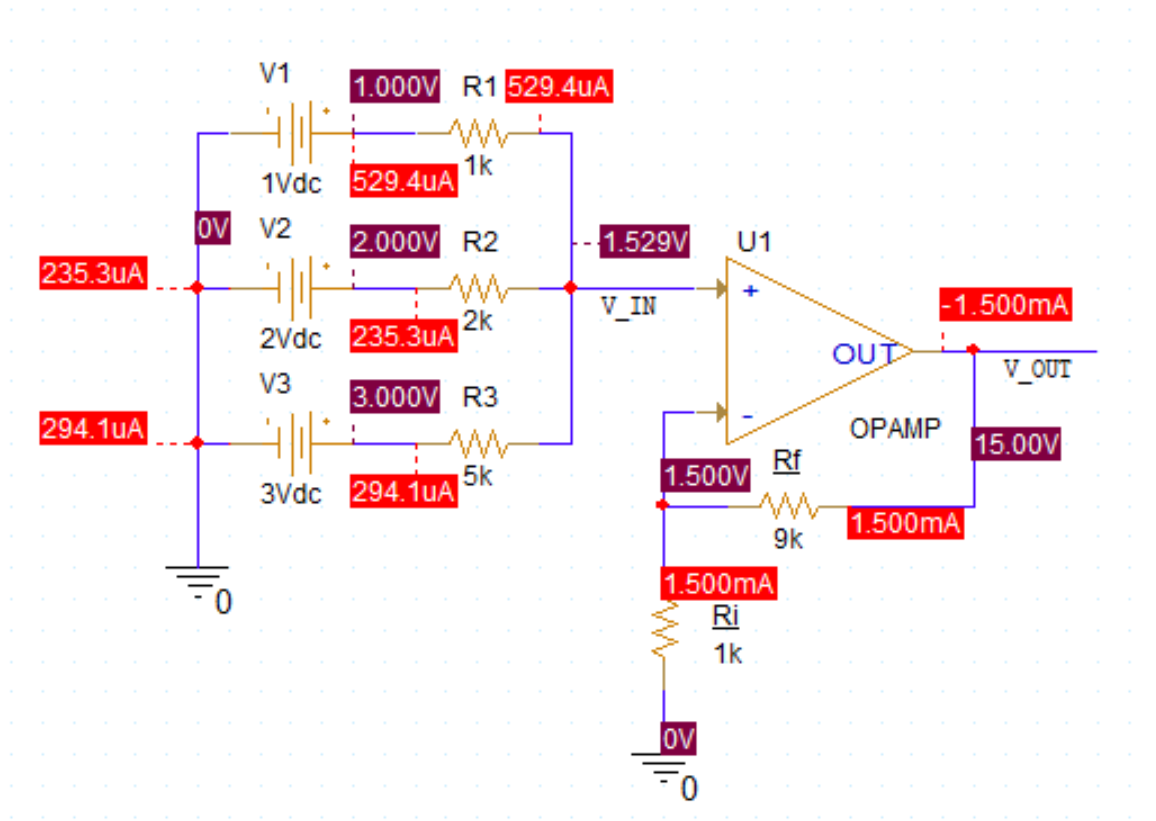
\includegraphics[width=0.84\textwidth]{graphics/ex1/f11.png}
    \caption{Non inverse summing using OPAMP}
\end{figure}
\pagebreak

\textbf{Giải thích}

Theo định luật Ohm, $I_{R_1} = \dfrac{V_{in} - V_1}{R_1}$, $I_{R_2} = \dfrac{V_{in} - V_2}{R_2}$, $I_{R_3} = \dfrac{V_{in} - V_3}{R_3}$

Theo KCL tại $V_{in}$, ta có: $I_{R_1} + I_{R_2} + I_{R_3} = I_{in}$ 

Mà $I_{in} \approx 0$ (Do theo mô hình lý tưởng của opamp điện trở đầu vào rất lớn)

Do vậy, $I_{R_1} + I_{R_2} + I_{R_3} = 0 $ hay $\dfrac{V_{in} - 1}{1k} + \dfrac{V_{in} - 2}{2k} + \dfrac{V_{in} - 3}{5k} = 0 \rightarrow V_{in} = \dfrac{26}{17} \approx 1.5294$ V.

Ta có opamp đang hồi tiếp âm và điện trở đầu vào rất lớn do vậy $V^- = V^+$ 

Theo định luật Ohm, ta có $\dfrac{V^- - 0}{R_i} = I_{R_f} = \dfrac{V_{out} - V^-}{R_f}$ (do dòng điện đi vào đầu âm của opamp gần bằng 0)

Do đó, ta có: $V_{out} = (1 + \dfrac{R_f}{R_i}).V^- = (1 + \dfrac{R_f}{R_i}).V_{in} = 10.\dfrac{26}{17} \approx 15,2941$ V

Nhưng $-V_{cc} \leq V_{out} \leq +V_{cc}$, $V_{cc}$ trong PSpice của Opamp là 15 V ($V_{NEG} = -15V$ và $V_{POS} = 15 V$) nên $V_{out}$ bão hòa ở mức 15 V.

Do vậy, $V_{out} = 15$ V suy ra $V^- = 1.5 V$

\begin{figure}[ht]
    \centering
    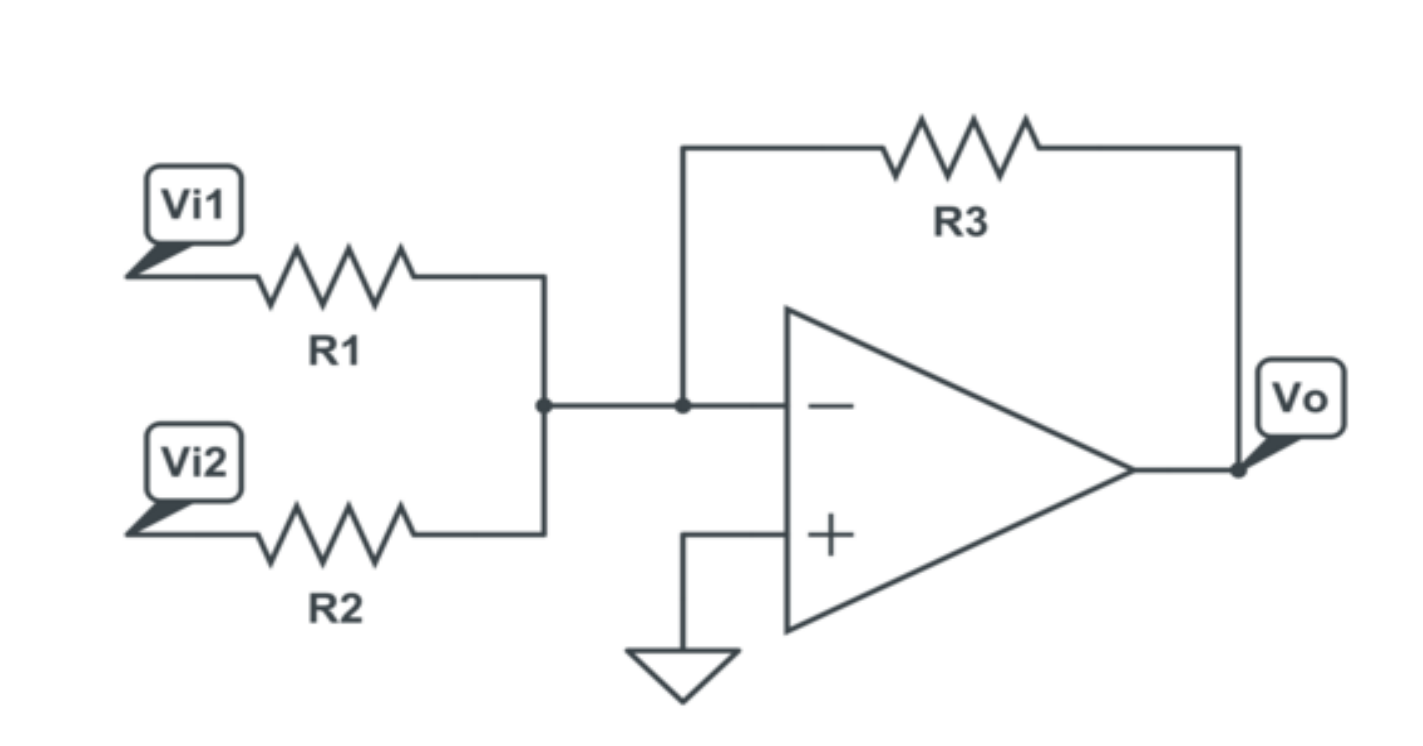
\includegraphics[width=0.6\textwidth]{graphics/ex1/f12.png}
    \caption{Inverse summing using OPAMP}
\end{figure}

The second type of the summing amplifier is proposed as follows:

Students are proposed to do the same steps above, with R1 = 1K, R2 = 2K, R3 = 10K and V1
= 1V, V2 = 5V.

\pagebreak

\textbf{Ảnh mô phỏng}

\begin{figure}[ht]
    \centering
    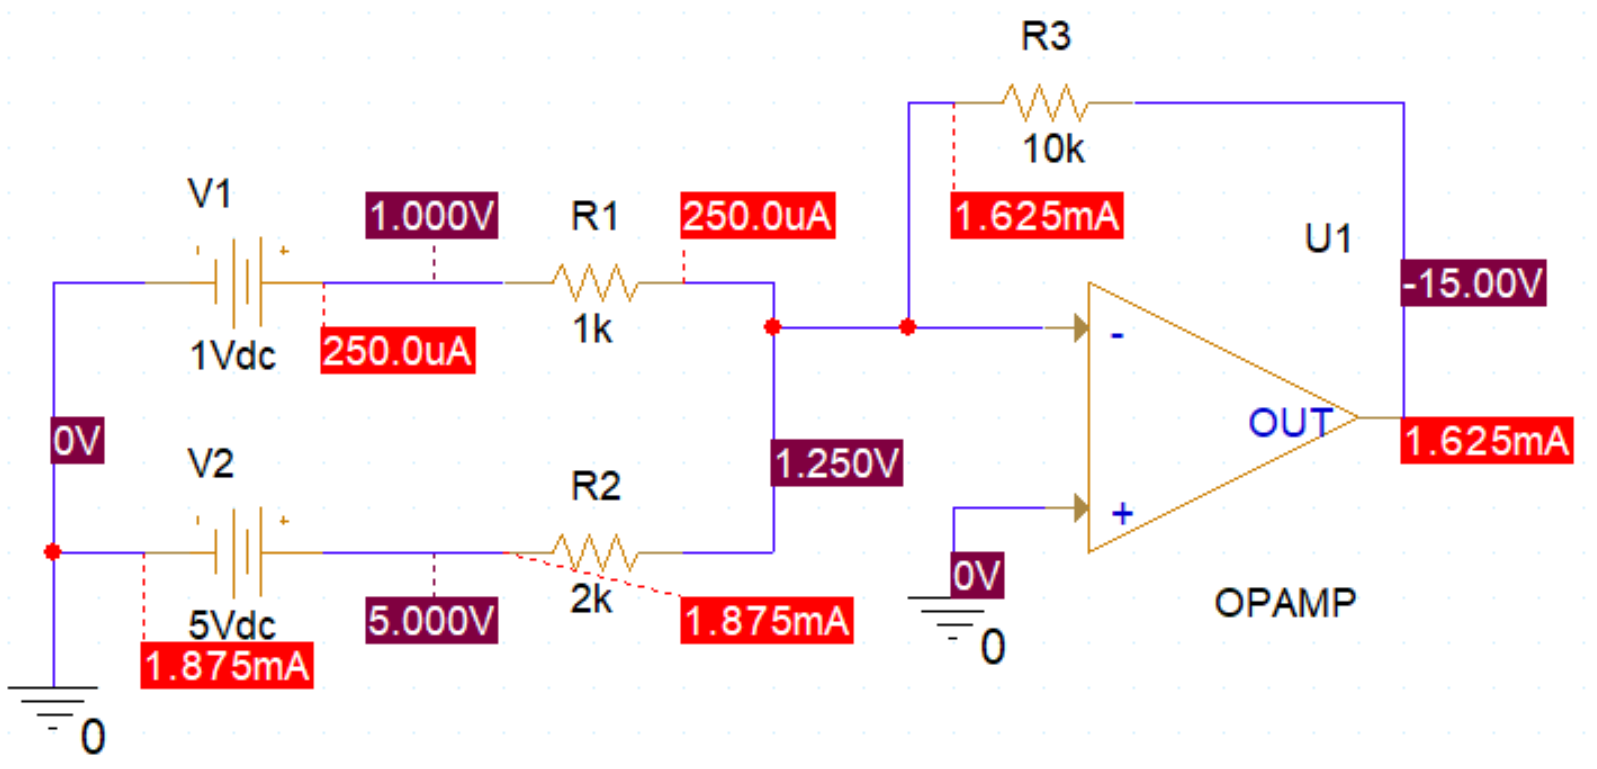
\includegraphics[width=1\textwidth]{graphics/ex1/f13.png}
    \caption{Inverse summing using OPAMP}
\end{figure}

\textbf{Giải thích}
Theo định luật Ohm và KCL tại đầu âm của Opamp, ta có: $I_{R_1} + I_{R_2} + I_{R_3} = I^- = 0$

Hay $\dfrac{V_1 - V^-}{R_1} + \dfrac{V_2 - V^-}{R_2} + \dfrac{V_out - V^-}{R_3} = 0$ (1)

Mà $V_{out} = A(V^+ - V^-) = -A.V^-$.

Do đó: $V^- = \dfrac{\dfrac{V_1}{R_1} + \dfrac{V_2}{R_2}}{\dfrac{1}{R_1}+ \dfrac{1}{R_2} + \dfrac{A+1}{R_3}} \approx 0$ (22) (Vì trong lí thuyết hệ số A rất lớn.)

Nhưng trong mô phỏng PSpice thì $A = 10^6$ và $V_{cc} = 15$ ($V_{NEG} = -15V$ và $V_{POS} = 15 V$). 

Từ (2) với $A = 10^6$, ta có: $V^- \approx 3,5.10^{-5}$ Nhưng $V_{out} = -A.V^- = -10^6.3,5.10^{-5} = -35 < -V_{cc}$

Do vậy, $V_{out}$ phải bão hòa ở -15 V. Từ đó (1) suy ra $V^- = 1.25$ V
\pagebreak

\subsection{Low Pass Filter}

Low pass filter is a filter which passes all frequencies from 0Hz (DC current) to upper cutoff frequency fH and rejects any signals above this frequency. A picture to demonstrate a
low pass filter behavior is shown in the figure bellow:

\begin{figure}[ht]
    \centering
    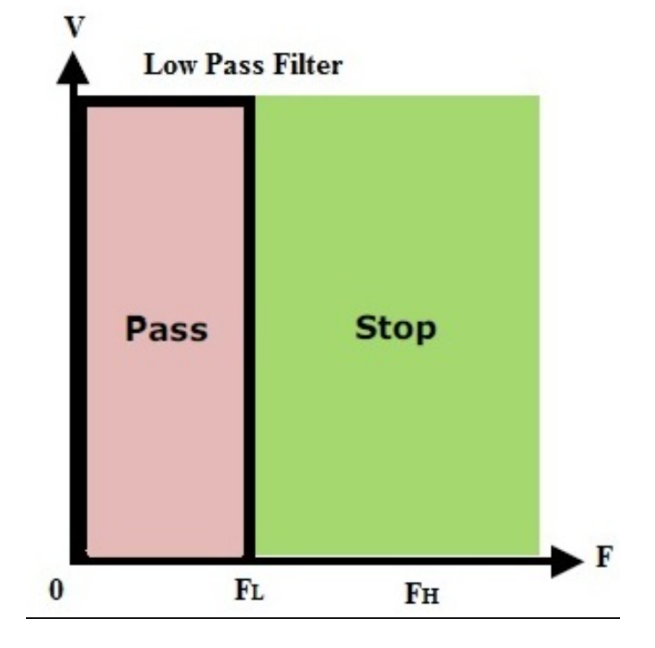
\includegraphics[width=0.4\textwidth]{graphics/ex1/f14.png}
    \caption{Low pass filter principles}
\end{figure}

Similar to the closed loop configuration, there also 2 types of low pass filter, including the
inverting and non-inverting low pass filter. The figure bellow is an inverting low pass filter.
The cut-off frequency is determined by this equation:
\[f_H = \dfrac{1}{2\pi R_2 C}\]

By applying the value of R2 = 10KOhm and C = 1nF, the cut-off frequency is around
16K Hz. In order to see the results, students are proposed to run the AC Sweep simulation profile (\textbf{Linear Type, Start and Stop frequency are 1Hz and 50kHz, 200 points}), as
follows:

\pagebreak
\begin{figure}[ht]
    \centering
    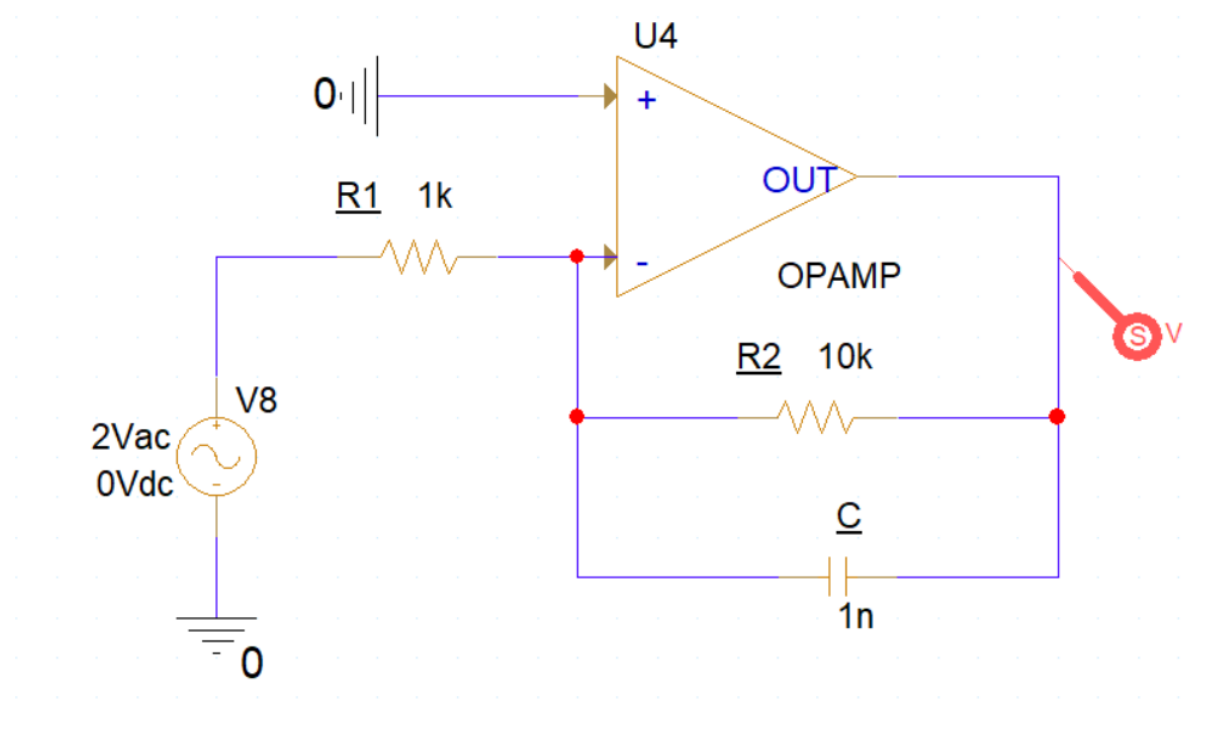
\includegraphics[width=0.77\textwidth]{graphics/ex1/f15.png}
    \caption{Inverting low pass filter}
\end{figure}

\begin{figure}[ht]
    \centering
    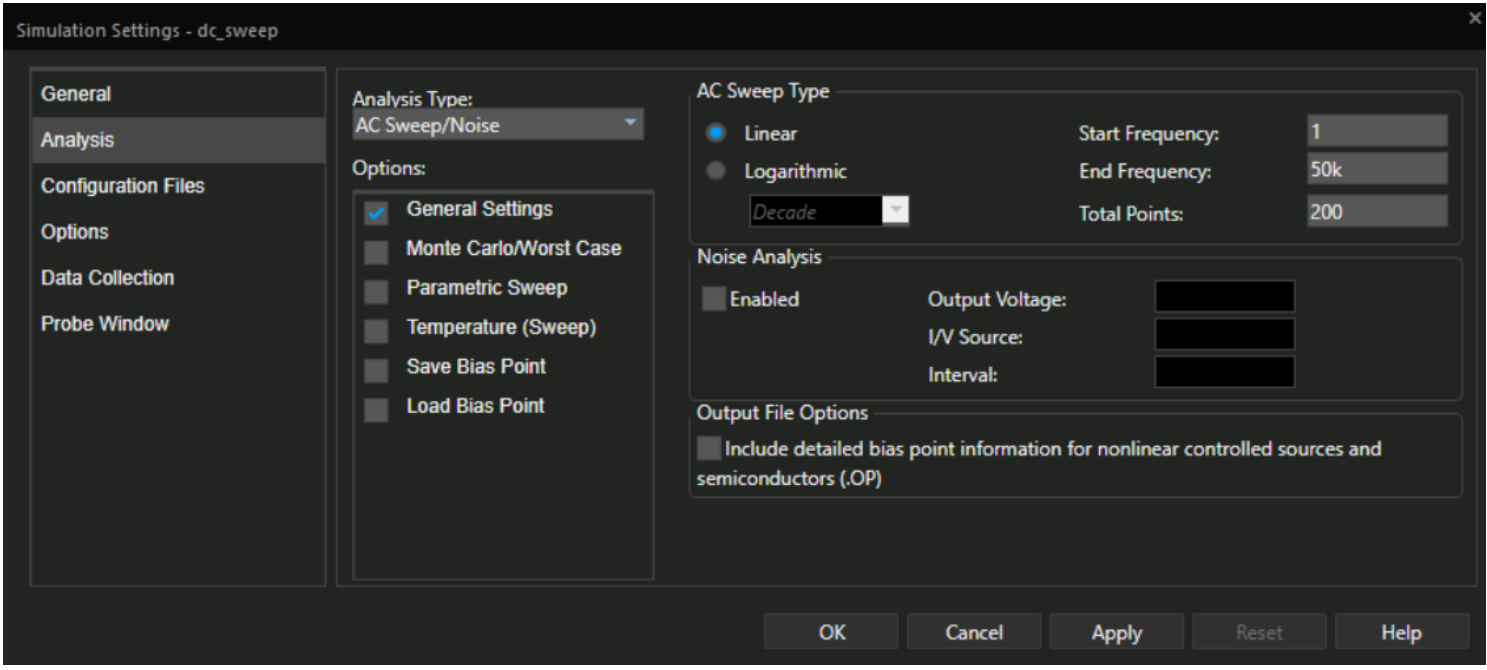
\includegraphics[width=0.88\textwidth]{graphics/ex1/f16.png}
    \caption{AC Sweep simulation profile}
\end{figure}

\begin{figure}[ht]
    \centering
    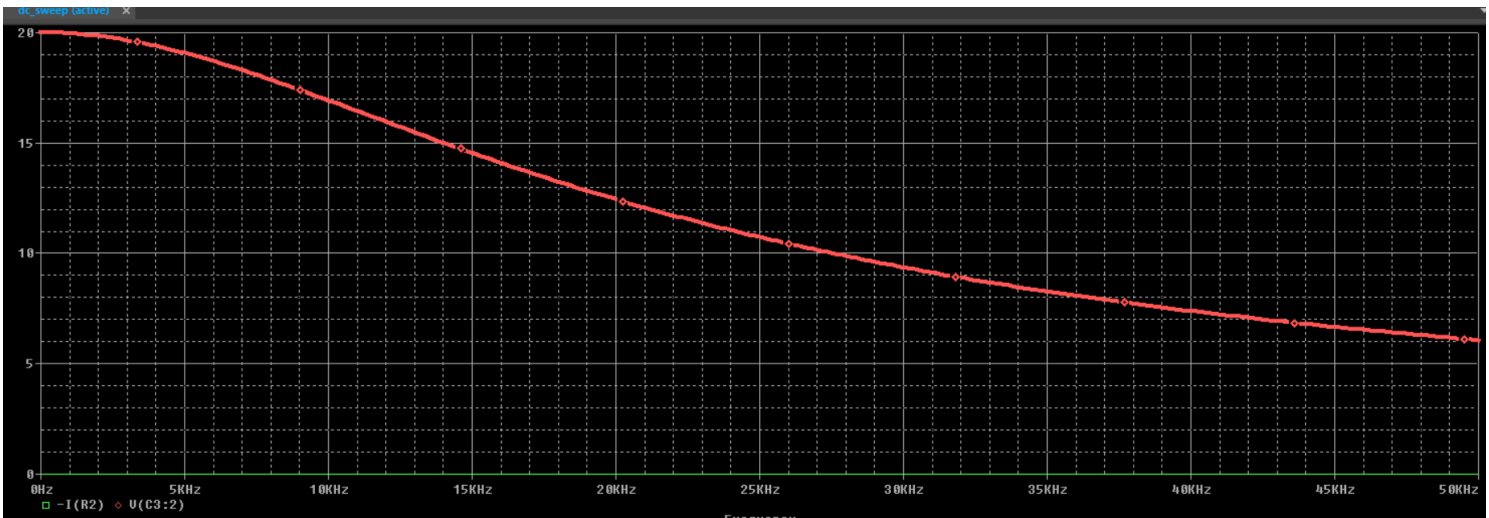
\includegraphics[width=0.8\textwidth]{graphics/ex1/f17.png}
    \caption{Simulation results}
\end{figure}

\pagebreak

The final results can be archived like the figure bellow:
It is said that the cut-off frequency point having the gain reduced 3dB. The gain at 0Hz
is 10 (input voltage is 2V and output voltage is 20V), or 20l og (10) = 20dB, meanwhile, the
gain at 16kHz is 7 (input voltage is 2V and output voltage is 14V), or 20l og (7) = 16.9.

The second type of a low pass filter, the non-inverting configuration, is presented as follows:

\begin{figure}[ht]
    \centering
    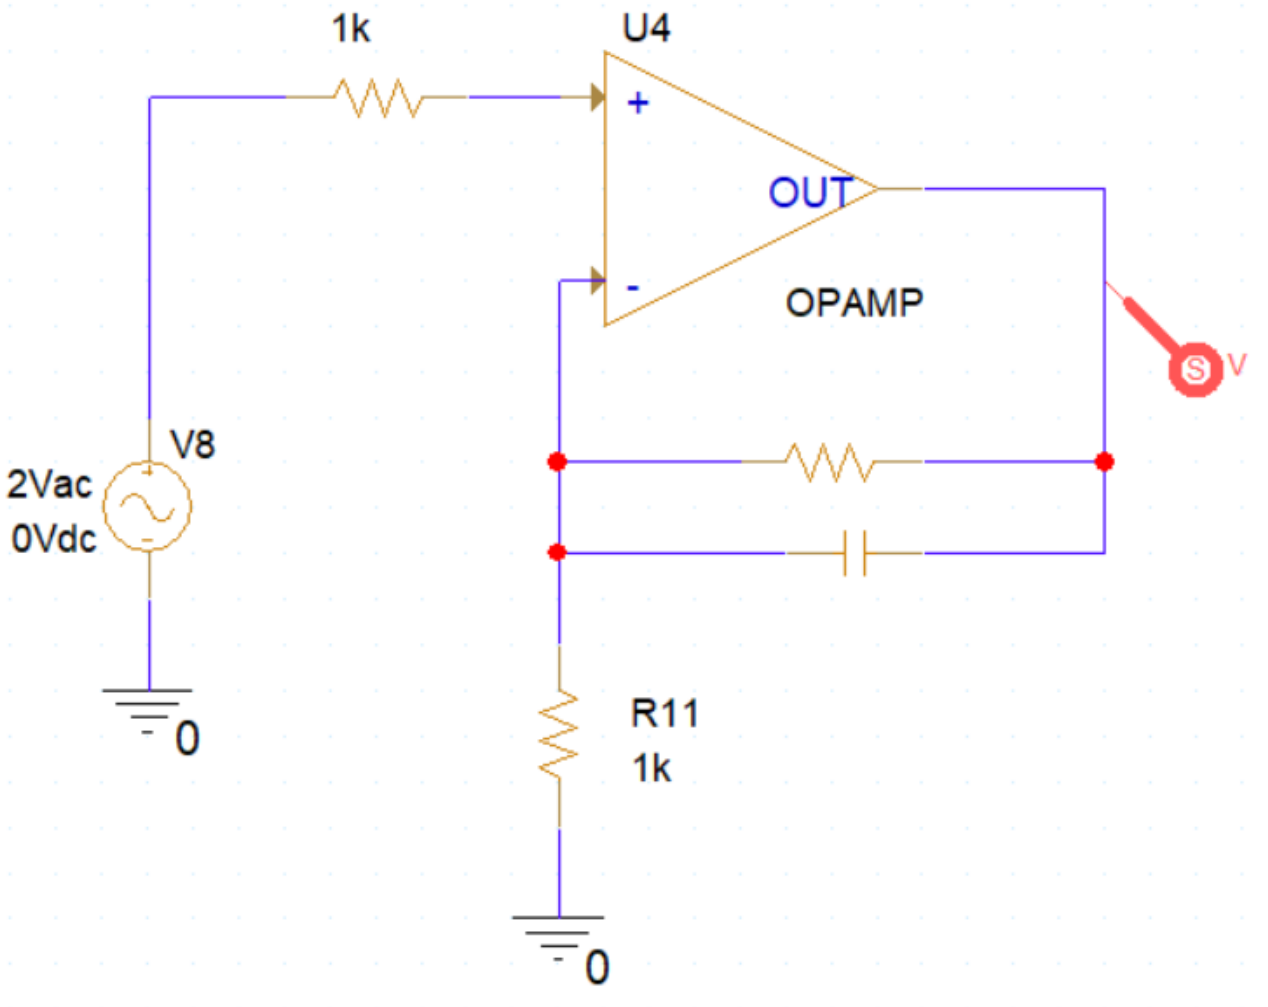
\includegraphics[width=0.6\textwidth]{graphics/ex1/f18.png}
    \caption{Non-inverting low pass filter}
\end{figure}

\textbf{Students are proposed to calculate the value of R and C to have the amplifier factor
equal to 10 and the cut-off frequency is the same as the previous example. The simulation result with AC Sweep mode is required to plot in this report as well.
}

\pagebreak

\textbf{Trả lời}

Ta có opamp hồi tiếp âm và điện trở đầu vào rất lớn, nên $V^+ = V^- = V_{in}$

Tại f = 0 Hz, theo định luật Ohm, ta có: $\dfrac{V^- - 0}{R_{11}} = I_{R} = \dfrac{V_{out} - V^-}{R}$

$V_{out} = (1 + \dfrac{R}{R_{11}}).V^- = (1 + \dfrac{R}{1k}). V_{in}$

$GAIN A = \dfrac{V_{out}}{V_{in}} = 1 + \dfrac{R}{1k}$

Để GAIN A = 10 tại f = 0Hz thì $1 + \dfrac{R}{1k} = 10 \rightarrow R = 9k$

Ta có $f_{H} = \dfrac{1}{2\pi RC} = 16 kHz \rightarrow C \approx 1.105 (nF)$

\textbf{Ảnh mô phỏng}

\begin{figure}[ht]
    \centering
    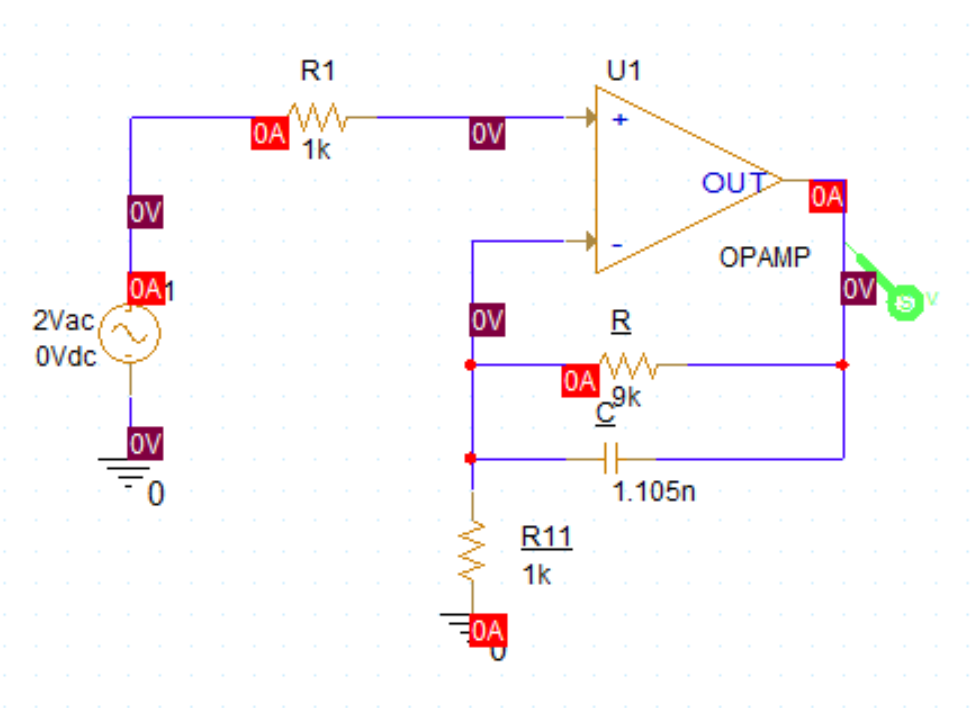
\includegraphics[width=0.7\textwidth]{graphics/ex1/f19.png}
    \caption{Non-inverting low pass filter}
\end{figure}
\pagebreak
\begin{figure}[ht]
    \centering
    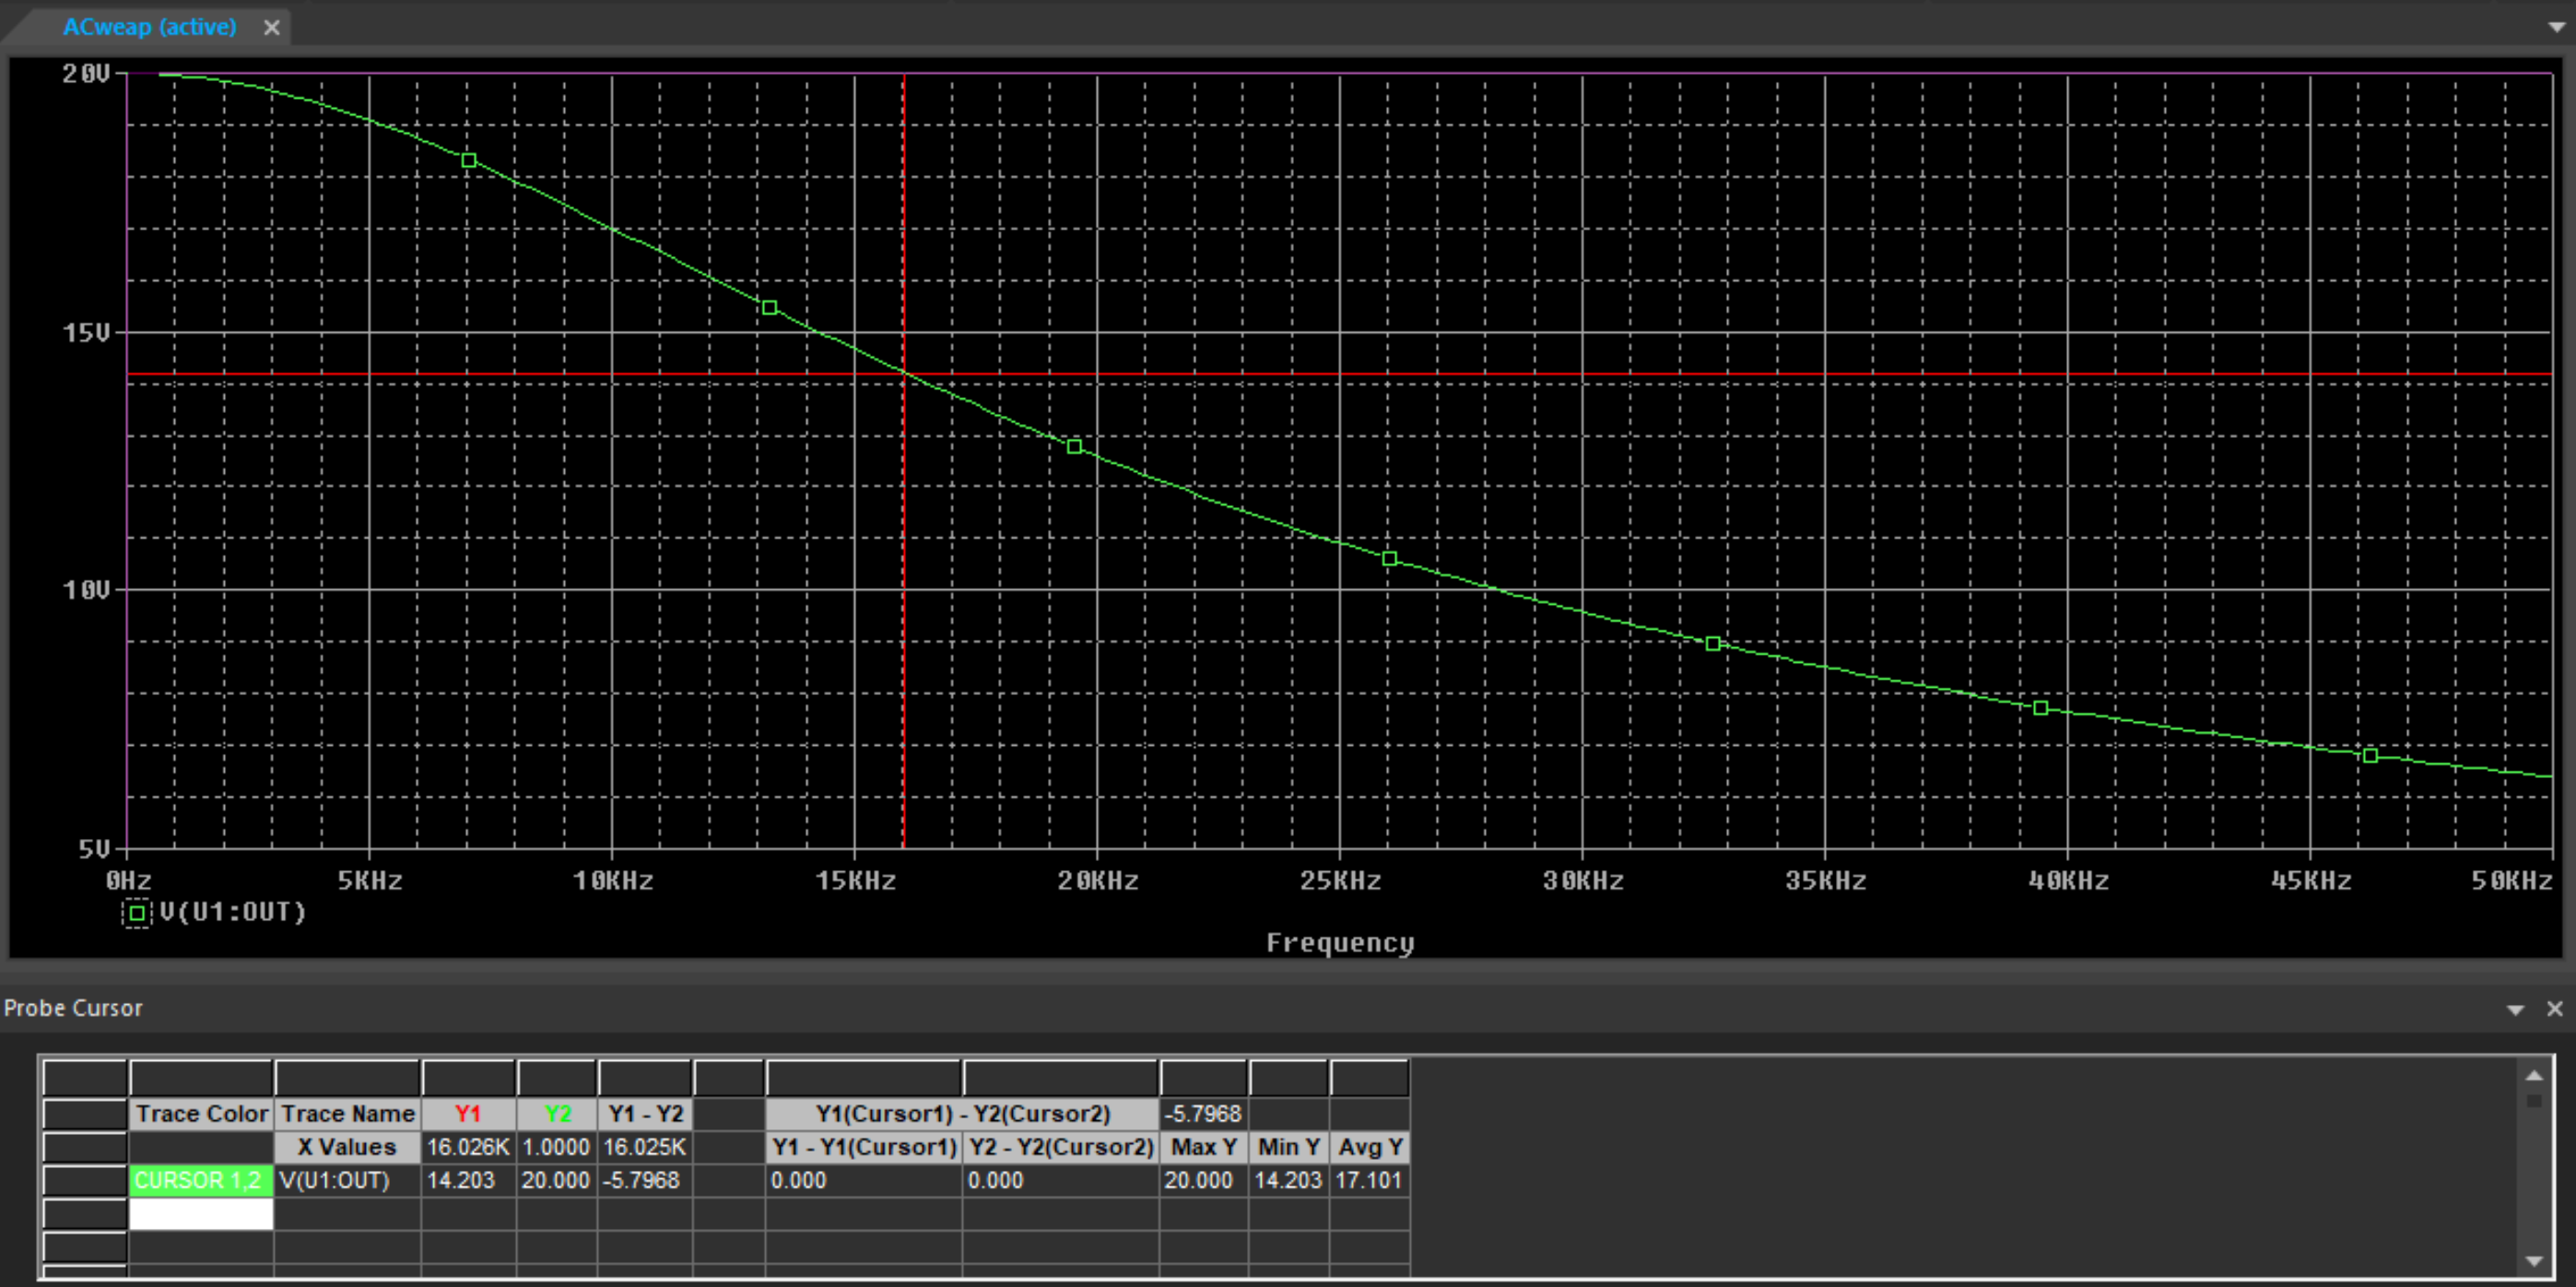
\includegraphics[width=1\textwidth]{graphics/ex1/f20.png}
    \caption{Simulation results}
\end{figure}

\textbf{Nhận xét:} GAIN tại f = 0Hz, $A = \dfrac{V_{out}}{V_{in}} = 10$ hay 20log(10) = 20dB. GAIN tại $f = f_{H} = 16kHz$, $A = \dfrac{V_{out}}{V_{in}} = \dfrac{14.203}{2} = 7.1015$ hay $20log(7.1015) \approx 17.027$ dB

Điểm tần số cắt có GAIN giảm 3dB.

\subsection{High Pass Filter}
In contrast to the low pass filter, there is a high pass filter, which can be referred from this
link:
\url{https://www.allaboutcircuits.com/video-tutorials/op-amps-low-pass-and-high-pass-active-filters/}
Students are proposed to implement a high pass filter in PSPICE and explain the behaviors
of your high pass filter.

\textbf{Trả lời}
\pagebreak

\textbf{Ảnh mô phỏng}

\begin{figure}[ht]
    \centering
    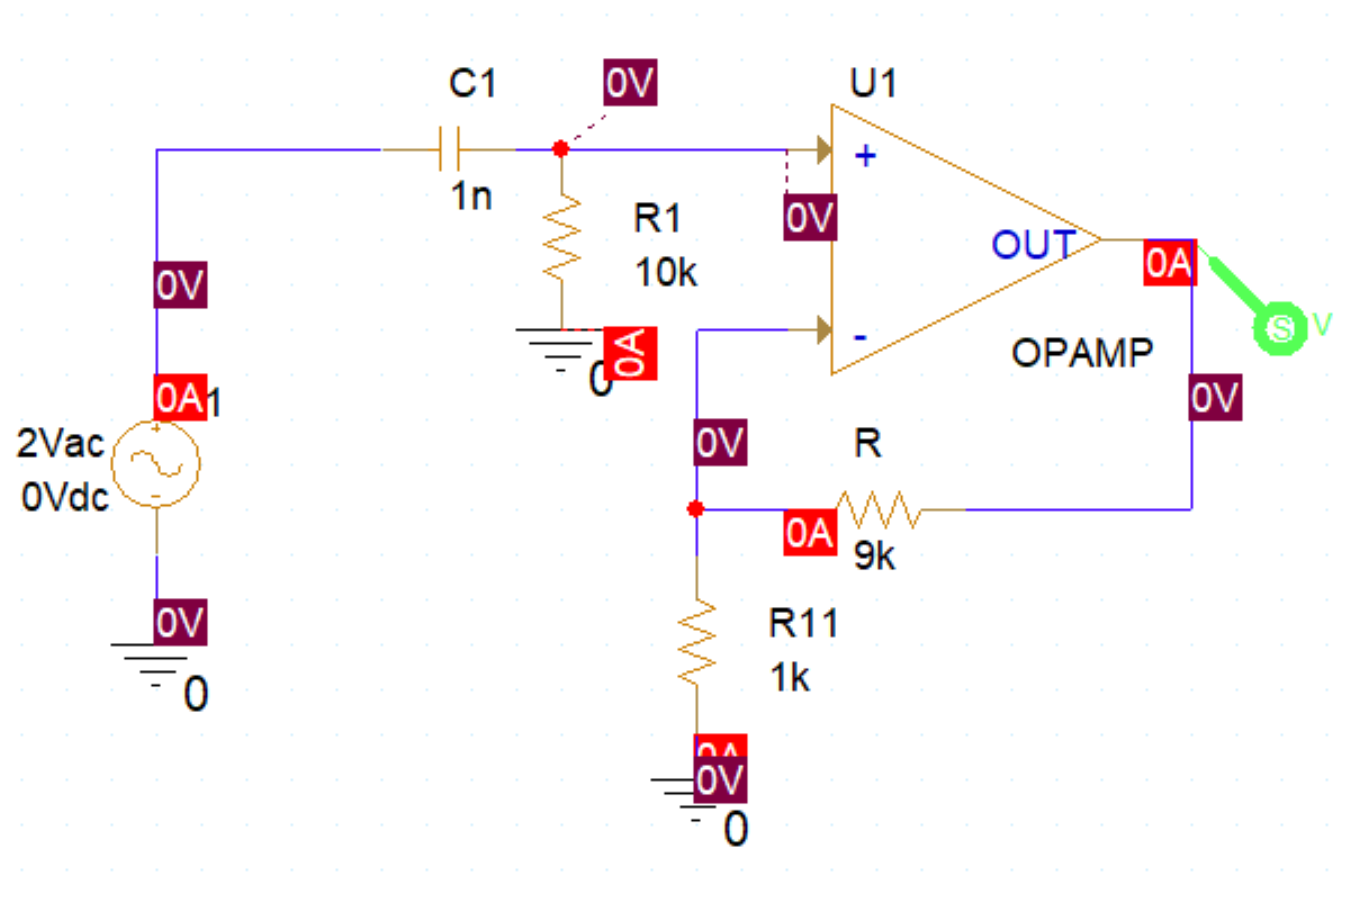
\includegraphics[width=0.7\textwidth]{graphics/ex1/f22.png}
    \caption{Non-inverting high pass filter}
\end{figure}

\begin{figure}[ht]
    \centering
    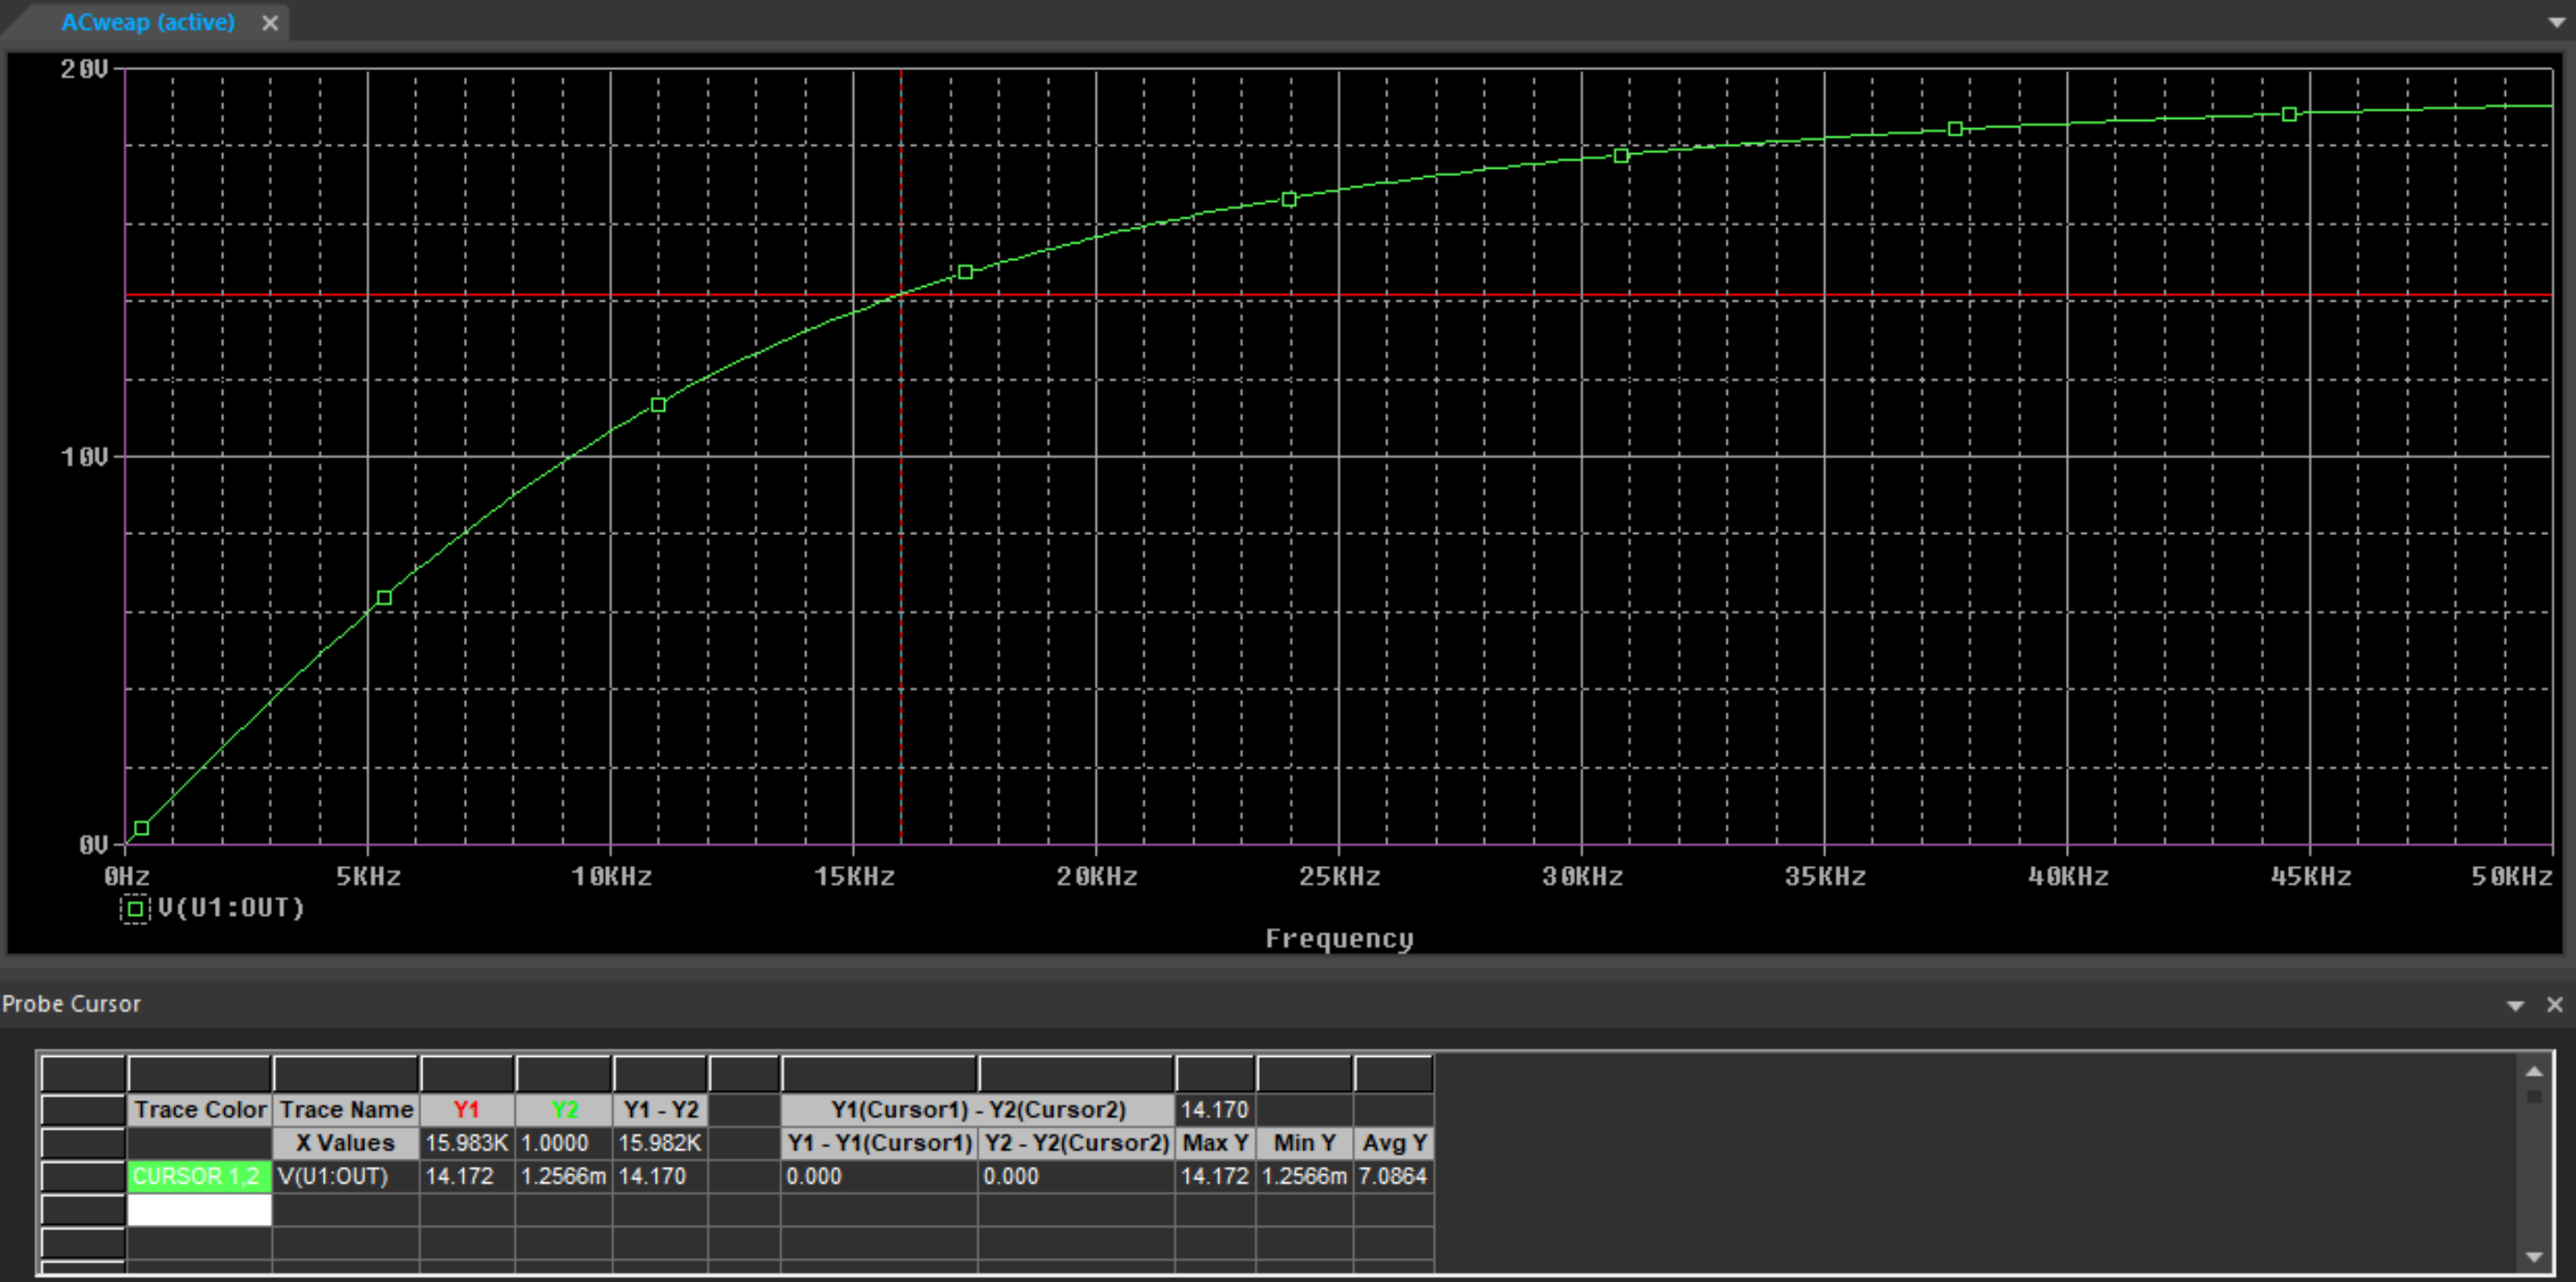
\includegraphics[width=0.9\textwidth]{graphics/ex1/f21.png}
    \caption{Simulation results}
\end{figure}
\pagebreak
\textbf{Giải thích} Ngược lại với bộ lọc thông thấp (low-pass filter), mức độ cản dòng của tụ điện là $Z_C = \frac{1}{2\pi fC}$ nên khi tần số nhỏ thì khả năng cản trở dòng điện của tụ lớn làm hạn dòng khiến biên độ dòng I nhỏ, điện áp vào opamp sẽ bằng dòng I.R1 khiến cho $GAIN = \dfrac{V_{out}}{V_{in}}$ (Vout là đầu ra của Opamp và Vin là tại nguồn dòng) giảm. Khi tần số tăng thì khả năng cản dòng của tụ cũng giảm đi khiến điện áp vào opamp, từ làm GAIN tăng. Còn GAIN của opamp khi tần số rất lớn sẽ là $GAIN = \dfrac{V_{out}}{V_{in}} = 1 + \dfrac{R}{R_{11}}$. Trong mô phỏng trên GAIN tại tần số rất lớn là 10 và tần số cắt của high-pass filter là $f_{L} = \dfrac{1}{2\pi R_1 C_1} \approx 16 kHz$. 

Như vậy khi tần số càng tăng thì GAIN càng tăng và tiệm cận đến 10. Tại tần số rất lớn thì GAIN = 10, tại f = 16kHz thì GAIN =  7.086, tại f = 0 Hz thì GAIN = 0. 

\subsection{Comparator with Hysteresis (Schmitt Trigger)}

The two resistors R1 and R2 act only as a "pure" attenuator (voltage divider). The input
loop acts as a simple series voltage summer that adds a part of the output voltage in series
to the circuit input voltage. This series positive feedback creates the needed hysteresis
that is controlled by the proportion between the resistances of R1 and the whole resistance (R1 and R2). The effective voltage applied to the op-amp input is floating so the op-amp must have a differential input.

\begin{figure}[ht]
    \centering
    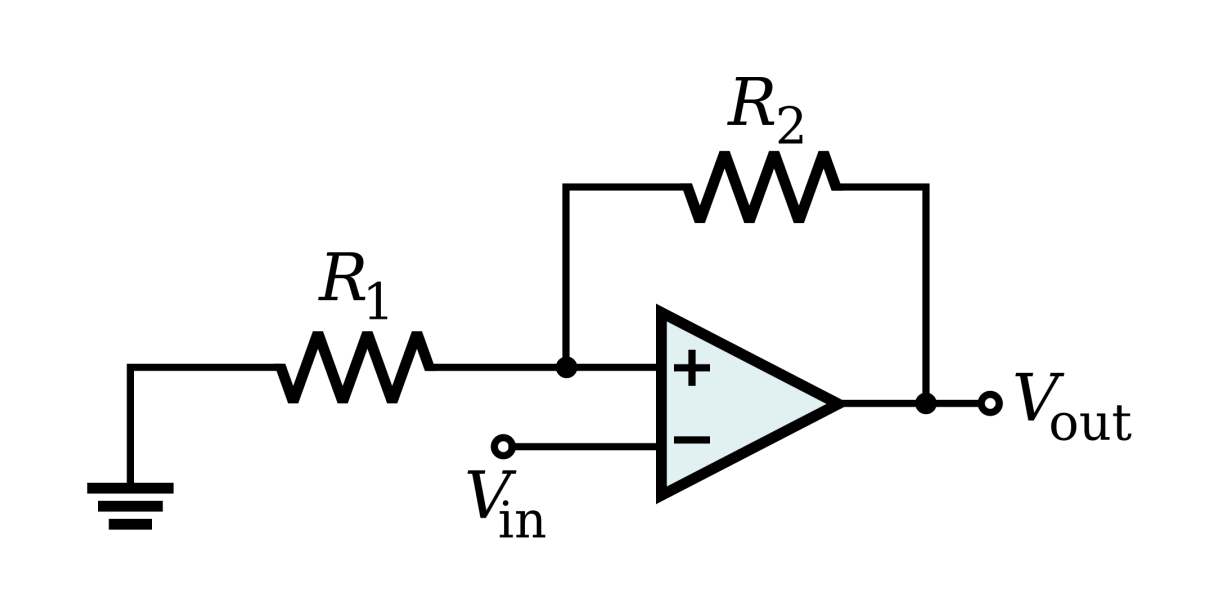
\includegraphics[width=0.55\textwidth]{graphics/ex1/f23.png}
    \caption{Inverting Schmitt trigger}
\end{figure}

The circuit is named inverting since the output voltage always has an opposite sign to the
input voltage when it is out of the hysteresis cycle (when the input voltage is above the
high threshold or below the low threshold). However, if the input voltage is within the
hysteresis cycle (between the high and low thresholds), the circuit can be inverting as well
as non-inverting. The output voltage is undefined and it depends on the last state so the
circuit behaves like an elementary latch.

In PSPice, this trigger is implemented as follows, with 3 voltage markers:

\begin{figure}[ht]
    \centering
    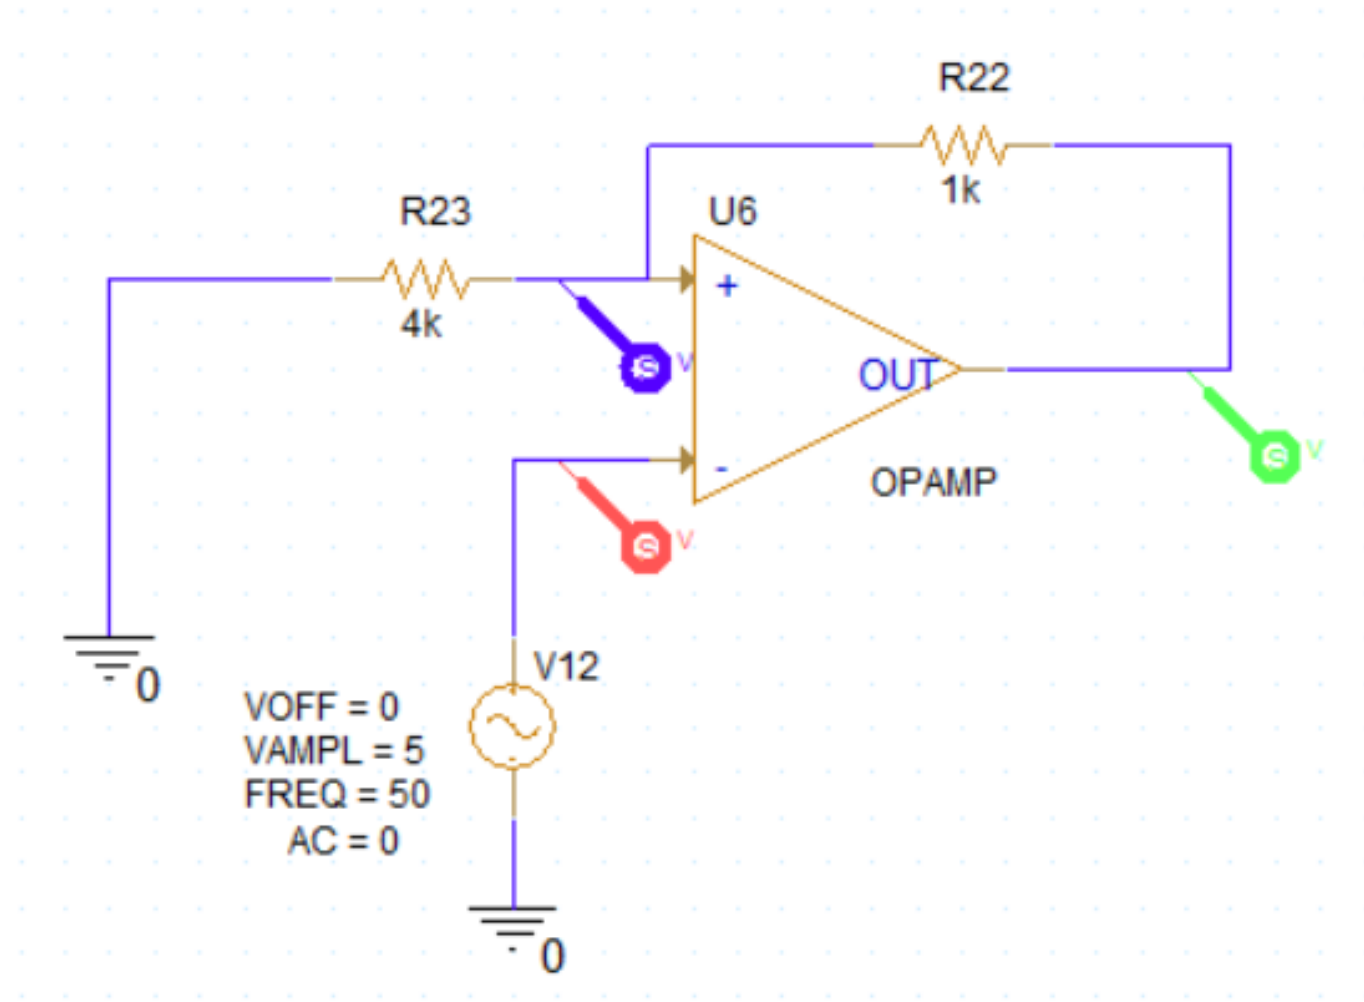
\includegraphics[width=0.55\textwidth]{graphics/ex1/f24.png}
    \caption{Inverting Schmitt trigger}
\end{figure}

The OPAMP device is modified in the \textbf{Properties} windows (right click on the component
and chose Edit Properties or double click on the component), in order to set the VPOS
and VNEG to +5V and -5V, as follows:

The simulation profile in this exercise is the \textbf{Time Domain}, and is configured as follows:
Finally, the simulation results can be archived as follows:

\textbf{Students are proposed to explain the signal at the output of the opamp. Why the signal
is toggled at +4V and -4V.}


\begin{figure}[ht]
    \centering
    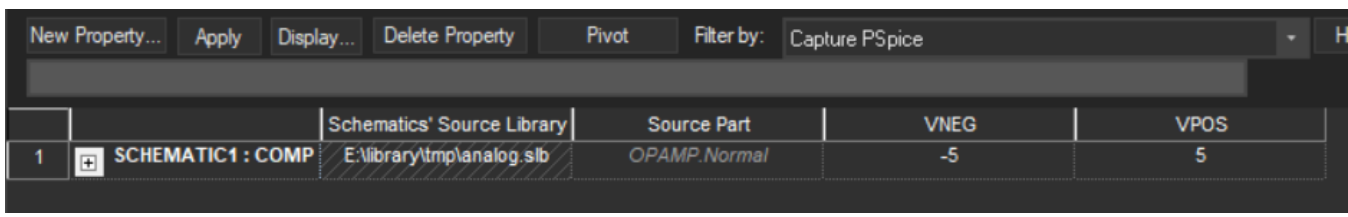
\includegraphics[width=0.66\textwidth]{graphics/ex1/f25.png}
    \caption{Schmitt trigger in PSPICE}
\end{figure}

\begin{figure}[ht]
    \centering
    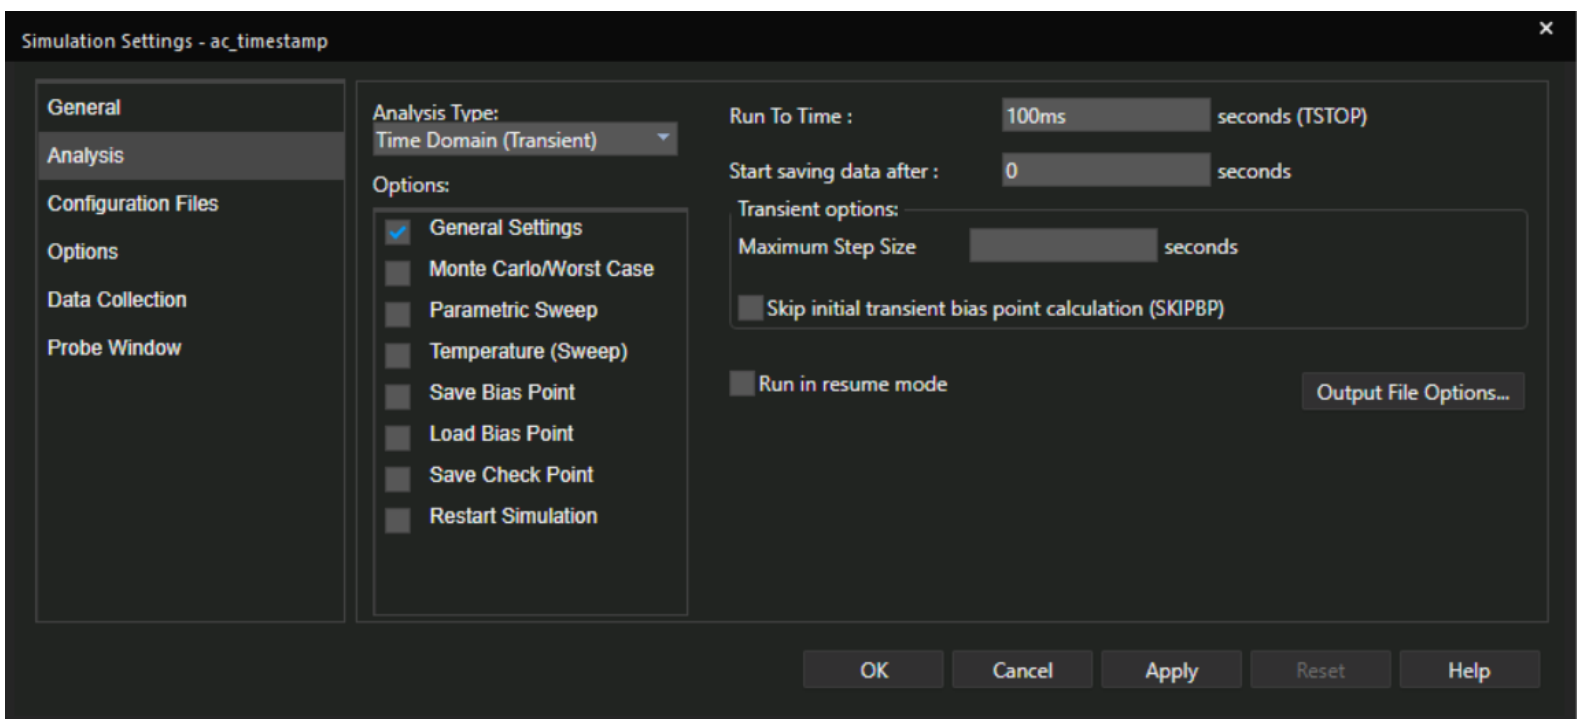
\includegraphics[width=0.6666\textwidth]{graphics/ex1/f26.png}
    \caption{Simulation profile}
\end{figure}
\pagebreak

\begin{figure}[ht]
    \centering
    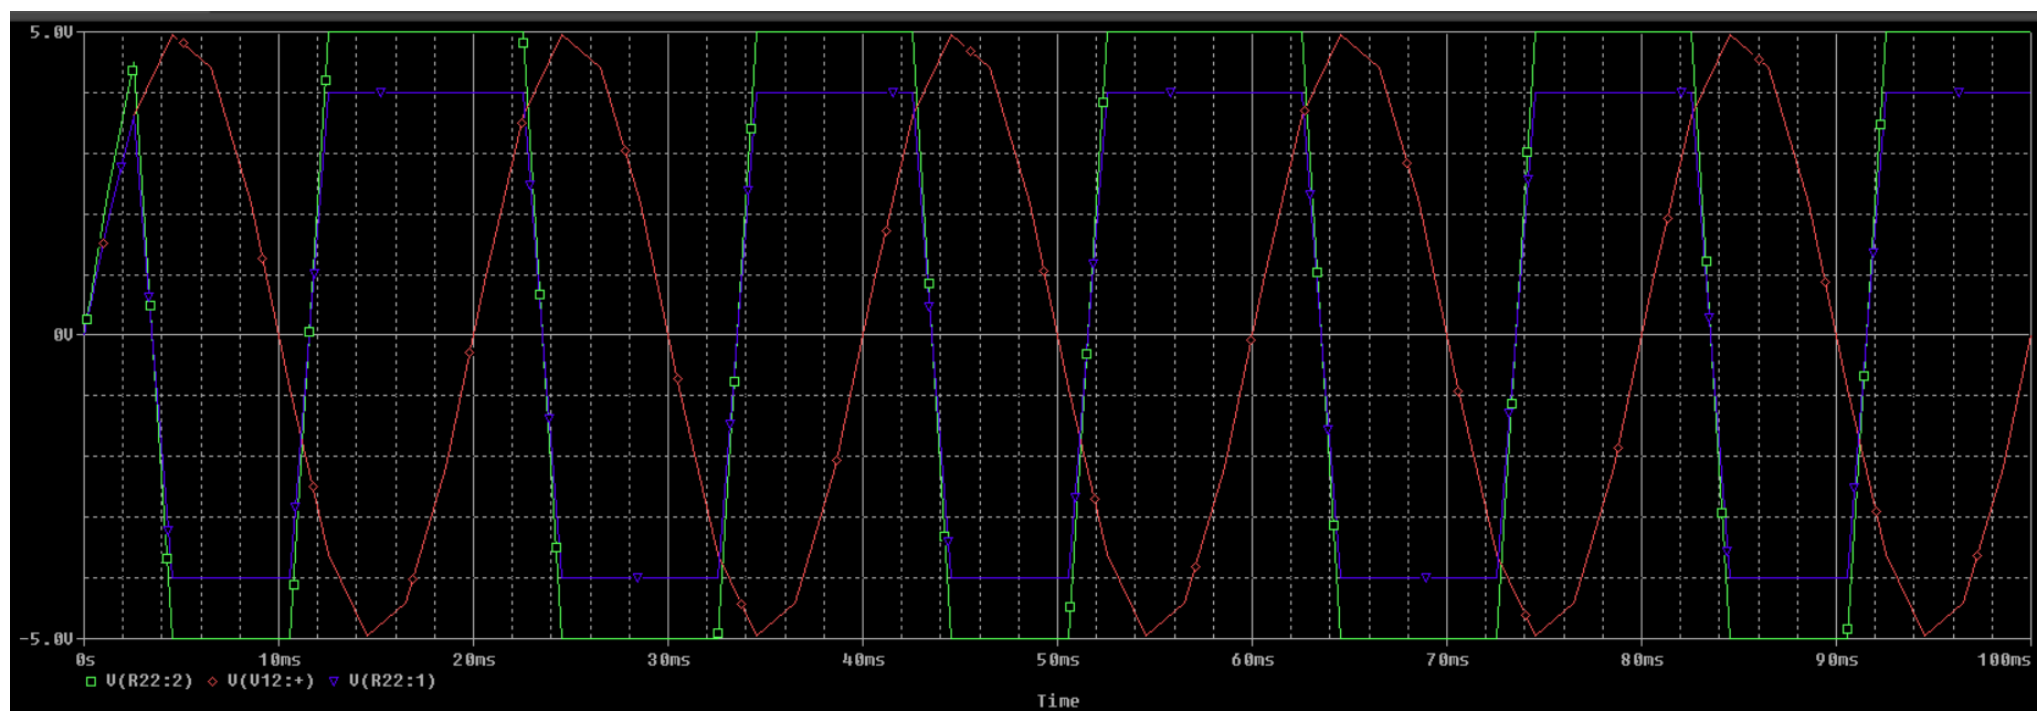
\includegraphics[width=0.66\textwidth]{graphics/ex1/f27.png}
    \caption{Schmitt trigger simulation results}
\end{figure}

\textbf{Trả lời}

Theo định luật Ohm, ta có: $\dfrac{V_{out} - V^+}{R_{22}} = I_{R_{22}} = \dfrac{V^+ - 0}{R_{23}} \rightarrow V_{out} = (1 + \dfrac{R_{22}}{R_{23}}).V^+$ (1)

Mà $V_{out} = A(V^+ - V^-)$

$\rightarrow V^+ = \dfrac{A}{A - 1 - \frac{R_{22}}{R_{23}}}.V^-$ hay $V_{out} = A(V^+ - V^-) = A(\dfrac{A}{A - 1 - \frac{R_{22}}{R_{23}}} - 1).V^- = \dfrac{A(1 + \frac{R_{22}}{R_{23}})}{A-1-\frac{R_{22}}{R_{23}}}.V^-$

Vậy $V_{out} = \dfrac{5}{4}.\dfrac{A}{A - 5/4} \approx \dfrac{5}{4}.V^-$ (do A rất lớn).

Nhưng trong mô phỏng trên PSpice, $V_{POS} = +5V$, $V_{NEG} = -5V$ nên $-5V \leq V_{out} \leq 5V$ nên khi biên độ của $V^- \geq 4V$ ($V^- \leq -4V$) thì $V_{out}$ sẽ bị bão hòa ở mức 5V (hoặc - 5V). Do đó nên điện áp tại $V_{out}$ sẽ chuyển đổi (toggled) ở mức -5V và +5V.

Theo (1), ta có: $V^+ = \dfrac{V_{out}}{1 + \frac{R_{22}}{R_{23}}} = \frac{4}{5}.V_{out}$ nên điện áp của $V^+$ sẽ chuyển đổi (toggled) ở mức -4V và +4V.


